% Tento soubor nahraďte vlastním souborem s obsahem práce.
%=========================================================================
% Autoři: Michal Bidlo, Bohuslav Křena, Jaroslav Dytrych, Petr Veigend a Adam Herout 2019

% Pro kompilaci po částech (viz projekt.tex), nutno odkomentovat a upravit
%\documentclass[../projekt.tex]{subfiles}
%\begin{document}

%===---------------====
% UVOD
%===---------------====
\chapter{Úvod}
\todo{Dopsat - az na konci}

%===---------------====
% TEORIE
%===---------------====
\chapter{Aspekty vývoje videoher}
Vývoj videoher je práce, jejíž výsledkem je hra na elektronické zařízení, jako například počítač, telefon, či konzole. Na jejím vzniku spolupracují umělci, designeři a programátoři, kteří mohou využít software vytvořený pro vývoj her\,--\,herní engine, který nabízí prostředky pro pohodlnější práci na vývoji her (viz kapitola~\ref{chap:Herní engine} Herní engine).

Proces vývoje videoher lze rozdělit na 7 základních etap: plánování, před-produkce, produkce, testování, před-spuštění, spuštění a post produkce~\cite{g2_game_development}.
\subsection*{Plánování}
V této etapě je vytvářen prvotní nápad na vývoj hry. Je základním kamenem a proto je velmi důležité důkladně vše promyslet a připravit, jelikož pozdější změny v plánu hry mohou mít drtivé dopady na celý vývoj~\cite{GameMaker_development}, jak časové, tak peněžní. 

Plánování je celé o pokládání a odpovídání si na otázky. Ty se můžou být obecné \uv{Jaký typ hry budeme vytvářet?}, \uv{Kdo bude cílové publikum naší hry?}, nebo se týkat příběhu hry: \uv{Jaká bude zápletka příběhu?}, \uv{Kde se bude hra odehrávat?}, \uv{Jaké postavy se budou ve hře nacházet?} a také technických parametrů hry: \uv{Pro jakou platformu budeme hru vytvářet?}, \uv{Jaké budou klíčové vlastnosti naší hry?}~\cite{g2_game_development}.

Pro takzvaný \uv{proof of concept}, díky kterému je zváženo, zda danou hru můžeme vytvořit je důležité najít a zanalyzovat otázky na odpovědi pro trh~\cite{GameMaker_development}. Těmi je například \uv{Kolik bude stát vývoj hry a jak tyto peníze získáme?}, \uv{Jak dlouho bude trvat vývoj?}, \uv{Máme potřebné zaměstnance a technologie na vývoj?} či \uv{Jakým způsobem hru zpeněžíme?}.

Cílem plánování je vytvořit základní koncept o čem hra bude, zjistit si cílový trh a~zhodnotit firemní zdroje a potenciály~\cite{novak2011game}.

\begin{figure}[hb]
    \centering
	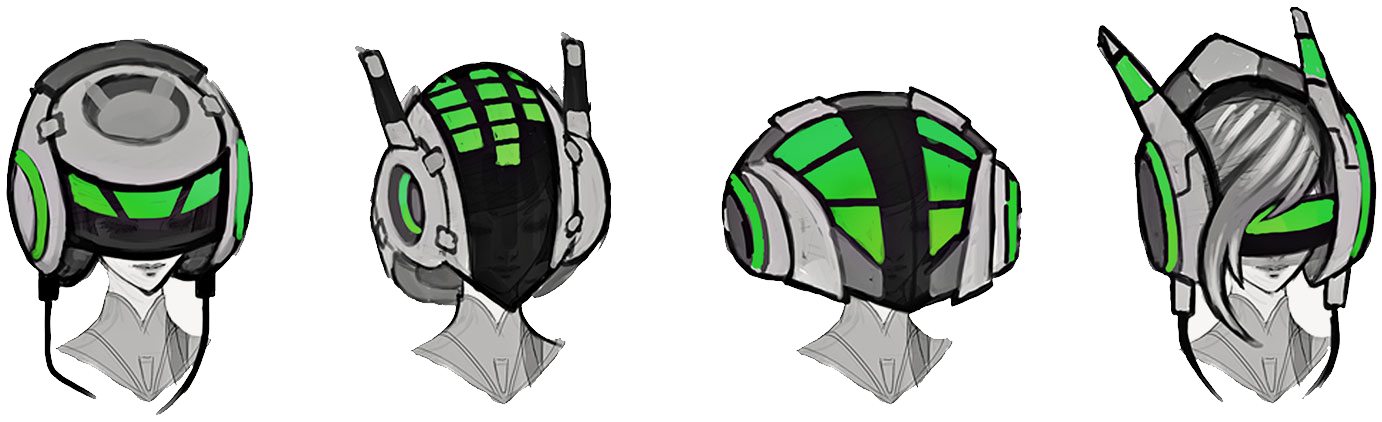
\includegraphics[width=0.95\textwidth]{obrazky-figures/ch2/concept_art.png}
	\caption{Concept art postavy ze hry League of Legends~\cite{artLOLvol1}.}
	\label{fig:concept_art_lol}
\end{figure}

\subsection*{Před-produkce}
Tato fáze přebírá odpovědi z plánování a rozšíří je o důležité detaily. Odehrává se při ní mnoho kolaborací mezi různými týmy (spisovatelé, programátoři, umělci, designeři, ...), aby se vyhovělo co nejvíce požadavkům a zabránilo se pozdějším komplikacím\,--\,programátoři například spisovatelům přiblíží technologické překážky platformy, které není možné překročit, či umělci a designeři navrhnou konzistentní barevné palety.~\cite{g2_game_development}.

Výsledkem před-produkce je dokument o herním designu (\textit{Game Design Document}, neboli GDD) a dokument technického návrhu a mohou zde být navrhovány první prototypy~\cite{novak2011game}. GDD je \uv{živý} dokument a vyvíjí se postupně po celou tvorbu hry\,--\,nalezneme tam detailní popis věcí jako například myšlenku hry, její žánr, celkový příběh, strategii monetizace, informace o postavách, základní herní mechaniky, design úrovní a světa, skici a \textit{concept arty}, neboli návrhy objektů/prostředí/postav~\cite{CG_Spectrum_GAMEDEVELOPMENT} (ukázka concept artu je na obrázku~\ref{fig:concept_art_lol}).

\subsection*{Produkce}
Nejdelší, nejdražší, nejnáročnější a nejdůležitější část vývoje~\cite{g2_game_development}, jejíž výsledkem je hotová hra. 

V této fázi je postupně vytvářen finální produkt. Jsou vymodelovány a animovány objekty, jako jsou postavy či prostředí, které jsou dále naprogramovány, čímž se přidají herní mechaniky a objekty jsou přivedeny k životu~\cite{GameMaker_development}. Tomu napomáhají i zvukoví designeři~a~dabéři, kteří se starají o audio stránku hry.

Při produkci nejsou neobvyklé změny, kde je nutné smazat i celé segmenty hry~\cite{g2_game_development}. Často se stává, že je nutné změnit nějaké natrhnuté či již vytvořené části, ať už je to kvůli nutnosti zmenšit pracovní zátěž vývojářského týmu, či kvůli zjištění, že neimplementovaný objekt do hry nesedí, či nefunguje podle původních představ\,--\,jako například postava \uv{Boatman} ze hry Spyro the Dragon (viz obrázek~\ref{fig:spyro_cut}), která byla změněna na postavu \uv{Ballonist}, nejspíše aby dávalo větší smysl cestování na ostrov v oblacích~\cite{GameMaker_development}.

\begin{figure}[hb]
    \vspace{0.5cm}
    \centering
    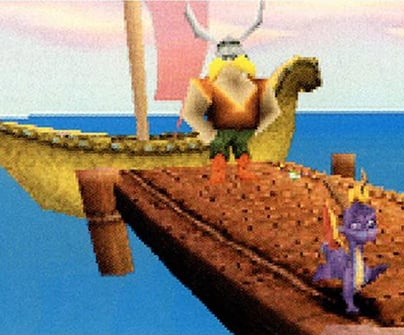
\includegraphics[width=0.5\textwidth]{obrazky-figures/ch2/Spyro-Boatman.png}\hspace{0.1cm}
    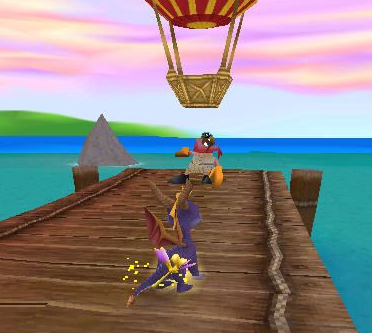
\includegraphics[width=0.46\textwidth]{obrazky-figures/ch2/Spyro-Ballonist.png}
    \caption{Postava Boatman (vlevo) ze hry Spyro the Dragon, který byl ve finální hře změněn na postavu Ballonist (vpravo)~\cite{GameMaker_development}.}
    \label{fig:spyro_cut}
\end{figure}

\subsection*{Testování}
Další důležitou fází je testování. V této fázi je důležité protestovat všechny možné problémy hry, které by mohli kazit zážitek ze hry.

Testy se dají rozdělit na 2 základní typy\,--\,testy technické stability a testování takzvaného \uv{fun factoru} hry, což je průzkum hratelnosti hry, její zábavnosti, poutavosti, a nebo zda není moc těžká, či lehká~\cite{GameMaker_development}. Testy technického faktoru zkoumají, zda se hra správně renderuje, neseká se, dále testeři vyhledávají různé bugy/chyby (např. zda opravdu nejde projít zdmi, nebo jestli se postavička projde místy, kterými by měla v pořádku projít), zda všechny funkce a postavy fungují tak jak mají a další podobné věci~\cite{g2_game_development}.

\subsection*{Před-publikace}
Fáze před publikací je marketingová. Je to období kdy se k veřejnosti dostanou trailery, teasery a demo verze hry~~\cite{GameMaker_development}. Díky tomu může hra získat větší fanouškovskou základnu a~vydavateli může dostat první zpětnou vazbu od veřejnosti.

\subsection*{Publikace}
Vypuštění a distribuce plné verze hry publiku.

Do spuštění hry musí být opraveno co nejvíce (při nejlepším všechny) chyb, proto často studia přichází s hierarchií chyb, které jsou potřeba opravit, od těch nejproblémovějších, které například rozbíjí hru, tak že často padá, až po ty nejdrobnější~\cite{g2_game_development}.

\subsection*{Post produkce}
V této etapě již hru vlastní a hraje veřejnost, často je ale vydáno zdarma několik dalších verzí hry (zvané \textit{patch}), které ji technicky vylepšují, vyvažují a často i opravují chyby~\cite{novak2011game}, na které se nedostalo při produkci, či které byly nově objeveny hráči. 

Také zde mohou přibýt \textit{updaty}, které do hry přidávají nový obsah (například události (\textit{eventy}), nové postavy/místa, atd.)~\cite{g2_game_development}. Nový obsah přidávají také rozšíření neboli DLC, které jsou ale často oproti updatům placené, nabízí více obsahu, a pro jejich spuštění vyžadují vlastní software (občas v kombinací s originální hrou) na spuštění~\cite{novak2011game}. Nový obsah udržuje hru relevantní~\cite{GameMaker_development}.

\subsection*{Milníky verzí vývoje her}
V průběhu vývoje videohra projde několika různými verzemi, které se od sebe liší jejich technickými vlastnostmi, kniha Game Development Essentials: An Introduction~\cite{novak2011game} uvádí nejdůležitější 3 z nich uvedené níže.
\begin{itemize}
    \item Alfa\,--\,v této fázi je již hra hratelná od začátku k cíli a je označována jako \textit{\uv{feature complete}}~\cite{CG_Spectrum_GAMEDEVELOPMENT}, což znamená že všechny hlavní vlastnosti jsou již implementované, nemusí zde být ale vše kompletně zoptimalizované. Měla by to být první verze testovaná lidmi mimo vývojářský tým.
    \item Beta\,--\,hra již v sobě má integrovaný všechen obsah, zaměření už je jen na opravě chyb a stabilizování projektu.
    \item Gold\,--\,finální dodělaná hra, která je připravena na publikaci.
\end{itemize}

%--------------------------
% Začátek videoher
\section{Začátek videoher}
První počítačové hry vznikaly kolem 50. let 20. století na vojenských základnách a univerzitách a jejich sálových počítačích~\cite{novak2011game}\,--\,těmito videohrami byla například OXO (1952), Tennis for Two (1958), ale do nepopulárnějších videoher (vytvořených v té době) se počítá hlavně hra vytvořena MIT studentem Stevem Russellem Spacewar!~\cite{bellis2019spacewar}, jenž je vidět na obrázku~\ref{fig:spacewar}. 


Nápad této hry byl následně, na začátku 70. let, přebrán Nolanem Bushnellem (zakladatelem Atari), který z ní vytvořil první komerční arkádovou hru (a tedy volně přístupnou veřejnosti) pod jménem \uv{Computer Space}, která byla velmi úspěšná~\cite{video_games_history}. To spustilo vývoj dalších velmi úspěšných arkádových videoher, oproti dnešním hrám převážně dovednostích, jako například \uv{Pong}, či \uv{Space Invaders} a \uv{Asteroids}, což byly první hry umožňující hráčům ukládat své skóre, dále například Galaxian, Pac-Man, Donkey Kong a Tron~\cite{novak2011game}.

Ve stejnou dobu začal i vývoj konzolových her, tedy možností hrát hry v pohodlí domova. Příklady firem, jejich konzolí a her (či herních sérií), které vznikli kolem této doby a zasloužili se o rozvoj konzolových/počítačových her, jako je známe dnes, jsou vypsány v~následujícím odstavci.
\begin{itemize}
    \item Atari\,--\,roku 1976 vydali jednu z prvních konzolí Atari VCS/2600, která odstartovala velkoprodej domácích konzolí~\cite{novak2011game}. Tato konzole přišla s mnoha, pro svojí dobu, ikonickými hrami, které byly často předělané tituly známe z arkád, jako je například Pac-Man série, Space Invaders, Asteroids, Q*bert, Pole Position či Frogger~\cite{Atari_games}.
    \item Nintendo\,--\,jejich první konzole, NES, byla vydána roku 1985. Vyšlo na ni mnoho dodnes populárních herních titulů, jako je například The~Legend of~Zelda, Super Mario Bros, Final Fantasy, Dragon Quest nebo Tetris~\cite{NES_GAMES}.
    \item Sega\,--\,jejíž první konzolí byla SG-1000 z roku 1983 s nejpopulárnější vydanou sérií Sonic the~Hedgehog~\cite{SegaRetro_2023}.
\end{itemize}

S příchodem personálních počítačů do domácností se zvýšil zájem o hry, mnoho původně pouze univerzitních her, bylo adaptováno do personálních počítačů, což způsobilo úpadek placených arkádových her~\cite{novak2011game}. 

V dnešní době jsou možnosti pro hraní videoher ještě rozšířenější, od možnosti hrát na telefonech, vyvinutějších ručních konzolích, či pomocí virtuální reality.

\begin{figure}[H]
    \centering
	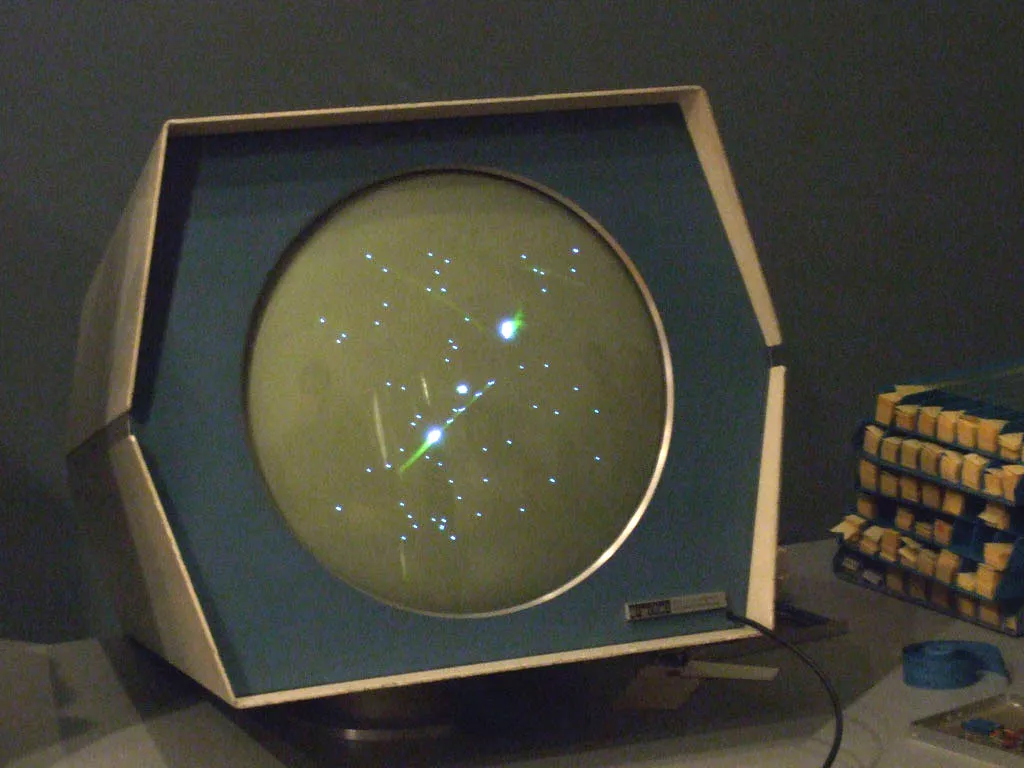
\includegraphics[width=0.53\textwidth]{obrazky-figures/ch2/Spacewar.png}
	\caption{Ukázka hry Spacewar~\cite{bellis2019spacewar}.}
	\label{fig:spacewar}
\end{figure}

%--------------------------
% Labyrintové hry
\section{Labyrintové videohry}
Dle Akademického slovníku současné češtiny~\cite{AkademickySlovnik-Bludiste} je bludiště, neboli labyrint, definováno jako \uv{místo, kde se bloudí} a \uv{složitý, neuspořádaný systém}. Bludiště jsou multikurzální, je to tedy spleť cest, chodeb a prostor, kde se snadno zabloudí a jsou definovaná slepými konci a~větvícími chodbami, kvůli kterým je procházející nucen se rozhodovat.

Andrew Rollings a Ernest Adams definují bludiště ve hrách jako prostředí, kde každé místo vypadá stejně, nebo velmi podobně a hráč musí zjistit, jak jsou místa propojená, často jejím procházením, aby našel cestu ven~\cite{rollings2003andrew}. Tyto hry jsou často doplněné o i nějaké výzvy než pouze procházení bludištěm, kterými, dle stejných autorů~\cite{rollings2003andrew}, může být například hledání klíče k otevření zamknutích dveří, sbírání věcí (např. pro zvýšení skóre), řešení hádanek, paměťových testů, luštění kryptických zpráv, atd.

V 80. letech 20. století měly hry s tématem bludiště největší rozmach, hlavně kvůli rozšíření domácích konzolí (např. Atari 2600), a díky jejich množství a rozmanitosti je lze rozdělit na 4 typy~\cite{DoYouMaze}:
\begin{itemize}
    \item bludiště s pohledem z vrchu\,--\,při hraní je vidět celé (či skoro celé) bludiště z vrchu (Mouse in the Maze, Bomberman),
    \item bludiště z prvního pohledu\,--\,stejný pohled na hru, jako herní postavička (Maze/Maze War, Capture the Flag),
    \item pronásledování bludištěm\,--\,hráč je pronásledován, či může pronásledovat nepřátele; tento typ je propojen s různými styly pohledu na bludiště (Pac-Man, Rally-X, Lady Bug),
    \item bludiště s obsazováním políček mřížky\,--\,hráč při průchodu bludištěm musí zabrat co nejvíce políček (Amidar).
\end{itemize}

\noindent Dále v textu se nachází příklady různých významných labyrintových her vytvořených v~průběhu historie.

\begin{figure}[H]
	\centering
	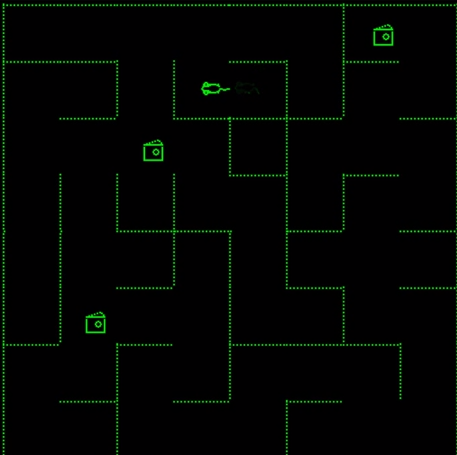
\includegraphics[width=0.5\textwidth]{obrazky-figures/ch2/MOUSE.png}
	\caption{Ukázka ze hry Mouse in the Maze.~\cite{Videogamehistorian}}
	\label{fig:mouse}
\end{figure}

\subsection*{Mouse in the Maze}
První labyrintovou hrou byla hra s názvem \textit{MOUSE}, nebo také \textit{Mouse in the Maze}, naprogramovaná roku 1959  Douglasem T. Rossem a John E. Wardem na sálovém počítači TX-0~\cite{TheOriginOfSpacewar}. 

Hráč dostal 8x8 mřížku a následně mohl světelným perem odmazat zdi a přidat sýr(y) (či v upravené verzi martini) a následně sledovat myš procházející bludiště, kde si pamatovala již prošlé cesty, a hledající sýr, který musela najít než se vyčerpala~\cite{Videogamehistorian}. Ukázka ze hry je zobrazena na obrázku~\ref{fig:mouse}, ze kterého je vidět, že hra je bludiště s pohledem z vrchu.

\subsection*{Maze/Maze War}
3D labyrintová pronásledující střílecí hra z roku 1974 vyvinutá studenty MIT~\cite{Maze_War}. Byla to průlomová hra, nabízející nejen iluzi 3D grafiky, ale i podporou hraní až pro 8 hráčů, či nehráčské boty a byla nejspíše jednou z prvních, či možná i první střílecí hrou~\cite{virtual_worlds}. Později byla hra díky využití TCP/IP protokolu, díky kterému hráči mohli hrát mezi sebou po internetu, průkopníkem i v online hrách~\cite{Maze_War}.

Úkolem hráčů, hrající jako avatar oční bulvy, bylo projít bludiště (kde mohli chodit pouze dozadu, dopředu a otáčet se o 90° vpravo, či vlevo), najít nepřátele a střelit je, čímž sbírali skóre~\cite{Maze_War}.

\subsection*{Pac-Man}
Japonská arkádová hra od společnosti Namco (dnes Bandai Namco Entertainment) vyšla původně v roce 1980 pod jménem Puck-Man (kvůli jeho tvaru puku, jméno ale bylo pro USA změněno, kvůli strachu z vandalů~\cite{kent2010ultimate}) a po svém vydání v USA se z ní stal okamžitý hit, neboť se v jednom roce prodalo více než 100 000 arkádových automatů s touto hrou~\cite{PACMAN}. Hitem byly i další hry z rychle rostoucí série Pac-Man. Roku 1981 vyšla Ms. PAC-MAN, jenž získala několik nových herních prvků, jako například více bludišť (oproti pouze 1, které nabízel originál) či náhodnější nepřátele\,--\,po svém vydání prodala i tato hra v USA více než 100 000 automatů, což žádná jiná hra v USA nedokázala~\cite{kent2010ultimate}.

\begin{figure}[hb]
	\centering
	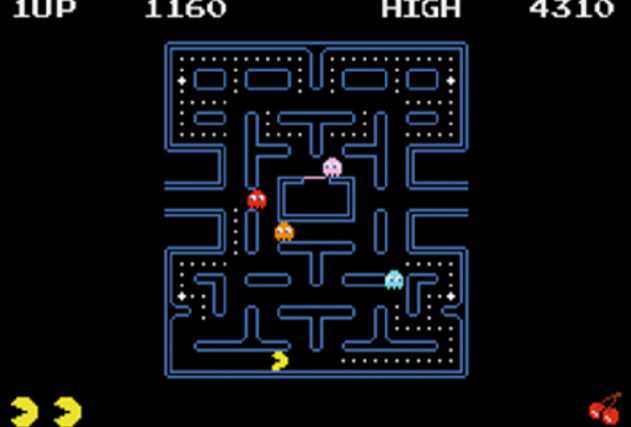
\includegraphics[width=0.7\textwidth]{obrazky-figures/ch2/pacman.png}
	\caption{Ukázka ze hry Pac-Man.~\cite{von2007space}}
	\label{fig:pacman}
\end{figure}

Pac-Man je hra založena na principu pronásledování hráče nepřáteli bludištěm~\cite{kent2010ultimate}, jak je vidět na obrázku~\ref{fig:pacman}. Hráč má za úkol projít bludiště a sebrat všechny tečky na zemi, čímž se dostane do další úrovně. Při tom ho ale pronásledují 4 duchové, kteří pokud ho chytí tak Pac-Man ztratí jeden ze 3 životů (když ztratí všechny, hra je prohraná). Hráč nadále může získat bonusové body díky sebranému ovoci, nebo pomocí bonusů, čímž se na omezenou dobu může nazpátek Pac-Man pojídat duchy.

\subsection*{Bomberman/Dyna Blaster}
Další labyrintová hra od japonských vývojářů, která je podobně jako Pac-Man, populární a vydávaná dodnes je Bomberman, v Evropě známý pod názvem Dyna Blaster, vydaný v roce 1983 (1985 na Nintendo konzole), kterého se prodalo za několik prvních let skoro milion kopií~\cite{Bomberman}. 
Mapa hry je jednoduchý obdélník s několika systematicky rozdělenými nerozbitnými zdmi, mezi nimiž se nachází volná místa a rozbitné zdi. Hráčův úkol je zničit všechny nepřátele pomocí pokládání bomb, které po určitém čase vybouchnou v křížovém tvaru, čímž zlikvidují nepřátele a rozbijí zdi v jeho výbušné oblasti, a také odejít dveřmi, které jsou schované za jednou ze zničitelných zdí~\cite{Bomberman}. 

%--------------------------
% Herní engine
\section{Herní engine}\label{chap:Herní engine}
Herní engine (také game engine) je softwarový framework využívaný pro tvorbu a vývoj (nejen) videoher. Nabízí mnoho nástrojů pro zjednodušení tvůrčího procesu, jako jsou například podpůrné programy, knihovny, a některé poskytují i speciální programovací jazyky vytvořené specificky pro programovaní her v daném engine~\cite{Valencia-Garcia_2016}. V následující části textu jsou popsány a uvedeny některé příklady z nejpopulárnějších herních enginů (viz obrázek~\ref{fig:most_popular_game_engines}).
\begin{figure}[H]
    \vspace{0.5cm}
	\centering
	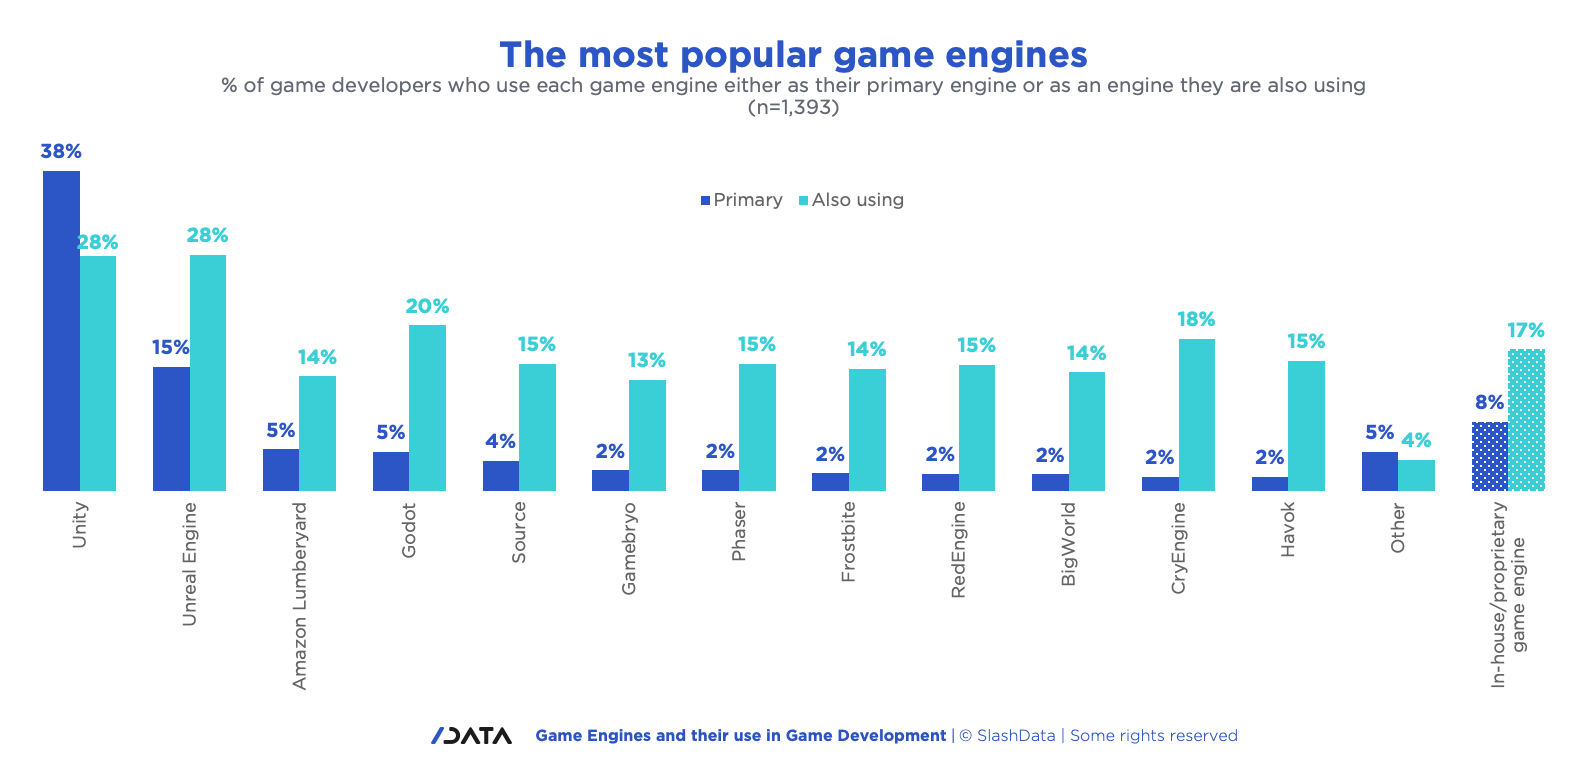
\includegraphics[width=\textwidth]{obrazky-figures/ch2/most_popular_game_engines.png}
	\caption{Výzkum SlashData z roku 2021 o nejpoužívanějších herních enginů.~\cite{SlashData_game-engines}}
	\label{fig:most_popular_game_engines}
\end{figure}

\subsection*{Unity}
Unity je multiplatformní game engine od společnosti Unity Technologies. Dle oficiálních webových stránek aktuálně podporuje více než 20 platforem (např. Windows, macOS, Linux, Android, PlayStation 5, Nintendo Switch,~\ldots)~\cite{unity_website}, nejen díky čemuž je jedním z~nejpoužívanějších softwarů na tvoření her~\cite{arnia_unity}. Poskytuje bezplatnou verzi (pro soukromé užití, nebo pokud výdělek hry za rok nepřesahuje 100 000\$) i placenou verzi \uv{Unity Pro}. 

Pro implementaci her, ať už 2D, 3D či VR (hry pro virtuální realitu), nabízí možnost vizuálního/grafického editoru a skriptů v C\#. Základní herní entita je \verb|GameObject|, které je množné přiřazovat různé vlastnosti, herní mechaniky, grafiku atd. a to již předefinované, či naprogramované uživatelem pomocí skriptů. Různé \verb|GameObjects| můžou být součástí \verb|Scene| z čehož je následně konstruován finální produkt~\cite{hocking2015unity}.

Unity je hojně využívána na vývoj AAA (také Triple-A hry neboli produkt od distributora, pro jehož vývoj byl k dispozici bohatý rozpočet) her, například: Marvel Snap, Apex Legends, ale i indie (takzvaně od nezávislých tvůrců = independent creator), například: Cult of the Lamb, Among Us, Slime Rancher, Cuphead~\cite{unity_website}.

\subsection*{Unreal Engine}
Unreal Engine je série herních engine, s nejnovější verzí Unreal Engine 5 z roku 2022, od společnosti Epic Games. První verze byla vytvořena pro tvorbu Unreal, 3D střílečky z pohledu první osoby, a byla velmi populární, jelikož díky UnrealScriptu (založeném na C++) mohli uživatele jednoduše původní hru modifikovat~\cite{sanders2016introduction}. Novější verze využívají klasické C++. Podobně jako Unity, nabízí bezplatnou i placenou verzi. Je také multiplatformní, ale podporuje menší škálu platforem než Unity\,--\,základní (Windows, Linux, PlayStation, Nintendo Switch, Xbox), ale podporuje~\cite{unreal_engine}.

V porovnání s dalšími zástupci herních engine je hodnocen jako jeden ze složitějších. Díky své komplikovanější stavbě a strmé křivce učení práce s Unreal Engine je doporučován spíše na větší, komplikovanější projekty, než například na mobilní hry (i přestože podporuje vývoj her na Android)~\cite{Kevuru_Games_Unreal-Unity}. Unreal Engine 5 je zaměřený hlavně na 3D vývoj a proto přišel s~mnoha funkcemi pro vylepšení vykreslování a práci s trojdimenzionálními objekty - jsou to Nanite (vizuální geometrický systém), Lumen (vylepšená práce se světlem) a MetaSounds (managment audia)~\cite{UnrealEngine5}.

Hrami, které byly vytvořeny za pomocí Unreal Engine je například Minecraft Dungeons, Final Fantasy VII Remake, Fortnite (ukázka na obrázku~\ref{fig:fortnite-unreal_engine}) nebo Stray~\cite{unreal_engine}.

\begin{figure}[H]
	\centering
	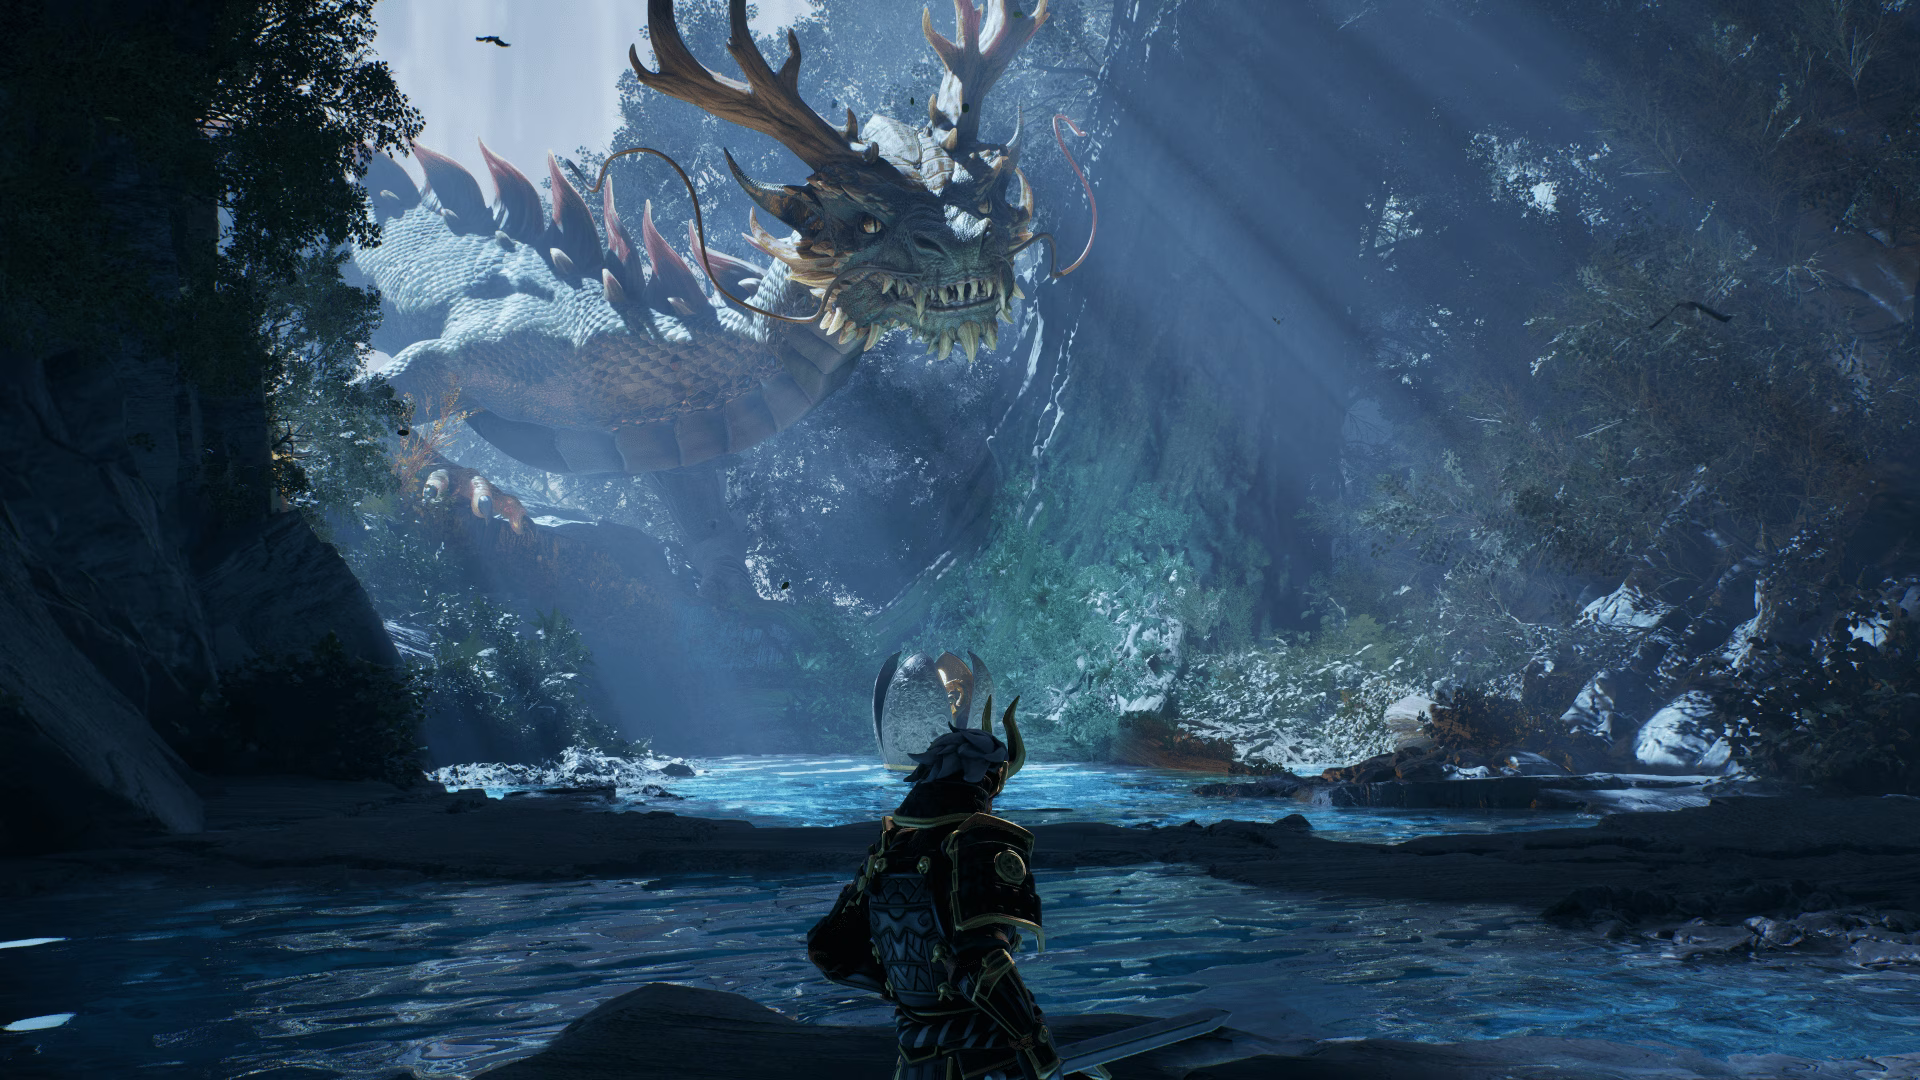
\includegraphics[width=0.66\textwidth]{obrazky-figures/ch2/fortnite.png}
	\caption{Ukázka ze hry Fortnite vytvořená pomocí Unreal Engine 5.~\cite{unreal_engine}}
	\label{fig:fortnite-unreal_engine}
\end{figure}

\subsection*{Godot}
Godot (s nejnovější verzí 4.2.1) je další software pro tvorbu 3D a 2D her. Na rozdíl od Unity a Unreal Engine je od verze 3.0 kompletně zdarma, svobodný a otevřený (open-source)\footnote{\url{https://github.com/godotengine/godot}}. Kvůli tomu má ale Godot oproti jiným zmíněným herním engine omezené oficiální možnosti platforem, jelikož jsou konzole (PlayStation, Xbox) uzavřené ekosystémy a Godot nimi není licencovaný~\cite{Godot_Engine_consoles}. Stále ale podporuje škálu platforem, příkladem desktopové (Windows, Linux, macOS), webové (HTML5), mobilní (Android, iOS) a virtuální realita (Oculus Rift/Quest, HTC Vive).

Základní stavební blok pro vytváření projektu v Godot je \verb|Node| (objekt reprezentující specializovaný prvek)\,--\,tyto objekty lze následně propojovat do \verb|Scene|, jak je vidět na obrázku~\ref{fig:godot_view}, což jsou stromy závislostí tvořící finální produkt~\cite{bradfield2018godot}. K těmto \verb|Nodes| lze přiřazovat skripty v jazycích GDScript (dynamicky typovaný jazyk syntaxí podobný Pythonu), C\# a C++\cite{GameEngineWizardry}. Godot se oproti předešlým zmíněným softwarům zaměřuje na 2D, pro které nabízí optimalizovaný přístup zdůrazňující jednoduchost a efektivitu (např. \verb|TileMap|, pro tvoření map, či \verb|Sprite2D| s vlastnostmi pro funkci 2D postav)~\cite{Godot_Engine}.

V Godotu byly vytvořeny například hry Brotato, Hive Time, Tail Quest a aplikace Dungeoncraft a Material Maker~\cite{Godot_Engine}.
\begin{figure}[H]
	\centering
	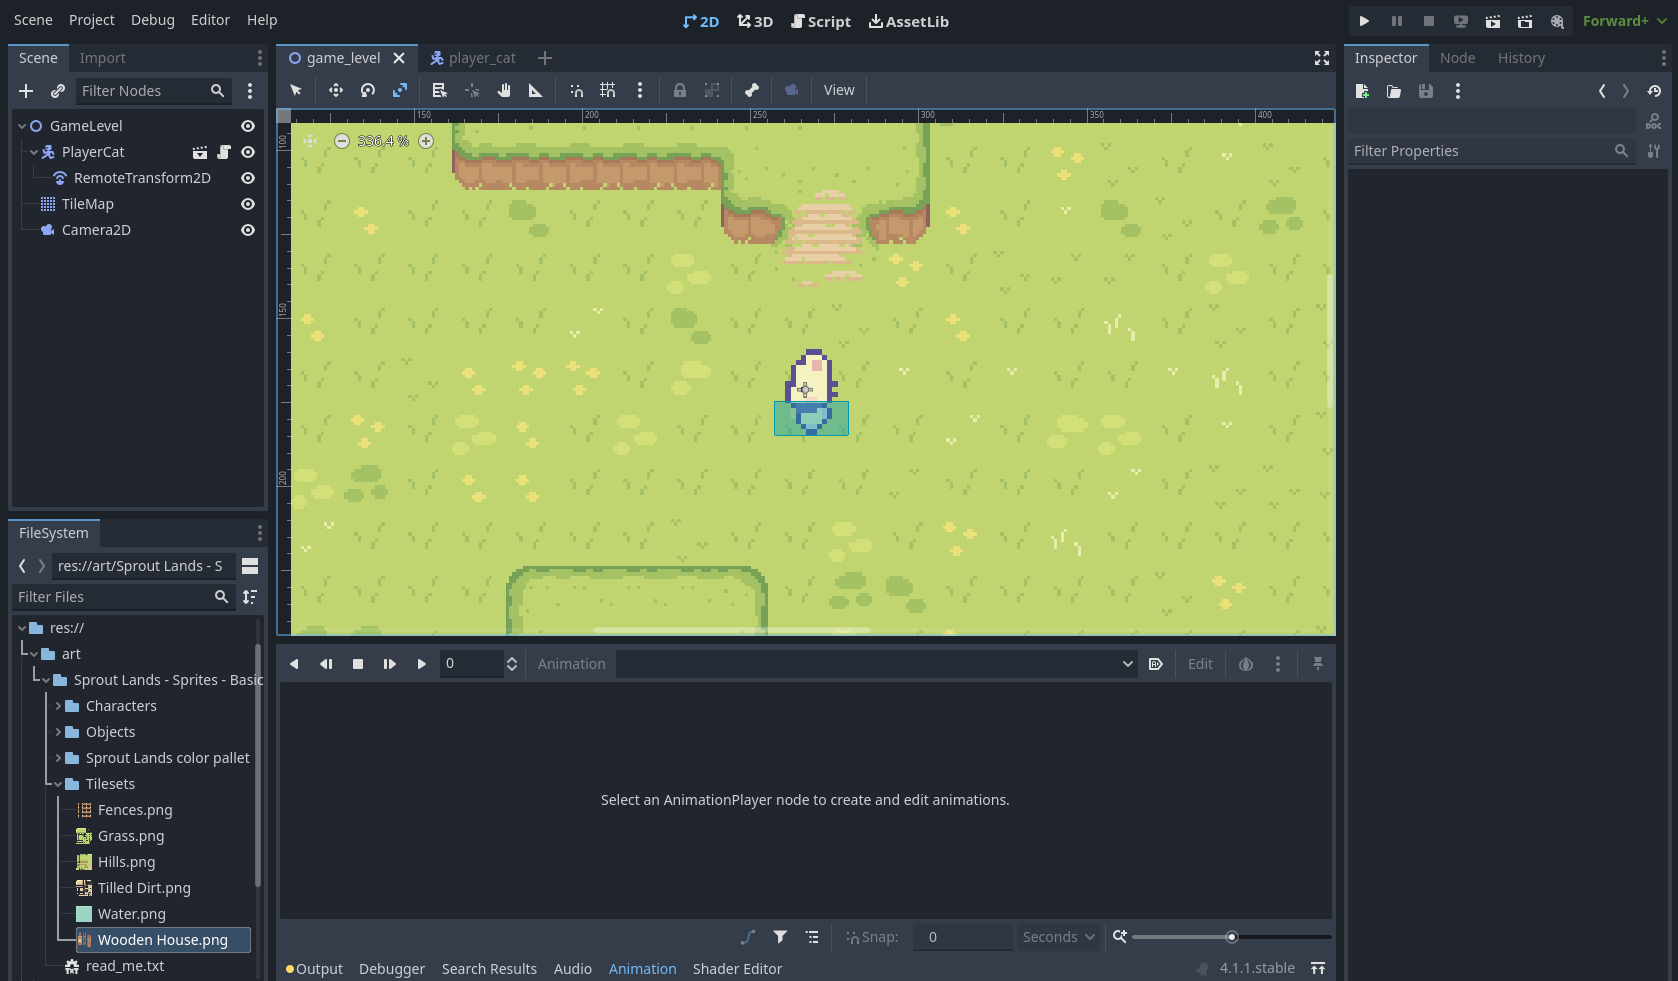
\includegraphics[width=0.8\textwidth]{obrazky-figures/ch2/godot_view.png}
	\caption{Grafické rozhraní pro zobrazení Scene v Godot verzi 4.2.}
	\label{fig:godot_view}
\end{figure}

%--------------------------
% Celulární automaty
\section{Celulární automaty}
Celulární automat (nadále označován také zkratkou CA) je dynamický systém a diskrétní model prostorového systému využívaný na modelování fyzikálních či biologických simulací. Prostorový systém vyjadřuje prostorovou dekompozici systému\,--\,zkoumaný systém je rozdělen na malé části s definovaných chováním~\cite{ims}.

\subsection*{Základní definice }
Celulární automat je čtveřice ${(\alpha^{n}, S, N, f)}$, kterou lze dle Stanfordské encyklopedie filozofie~\cite{sep-cellular-automata}, definovat následovně:
\begin{itemize}
    \item ${ \alpha^{n} }$ (\textit{Lattice}) je diskrétní n-dimenzionální mřížka buněk (${ n >= 1 }$)\,--\,tyto buňky jsou identické (některé mohou být speciální\,--\,např. modelují pevné hranice), 
    \item ${ S }$ je konečná množina stavů, které mohou buňky nabývat\,--\,v každém diskrétním časovém kroku může každá buňka nabýt pouze a jenom 1 stavu, 
    \item ${ N }$ je konečná množina sousedících buněk (okolí, které může, či nemusí obsahovat i~buňku samotnou) pro každou buňku, na kterém záleží její vývoj, ${ N \subseteq \alpha }$,
    \item ${ f }$ je konečná množina pravidel pro přechod mezi stavy\,--\,v každém časovém kroku každá buňka aktualizuje svůj aktuální stav podle deterministické přechodové funkce $\phi : \Sigma^n \rightarrow \Sigma$, která mapuje okolí. Často (i když ne nutně) se počítá, že aktualizace synchronní a bere jako vstup okolí v čase $t$ sousední stavy v bezprostředně předchozím časovém kroku $t-1$.
\end{itemize}
Příkladem zápisu definice celulárního automatu Game of Life (vysvětlený níže) lze zapsat jako:
\begin{equation*}
\begin{split}
    & \left( \alpha^{2}, \right. \\
    & \left. \{0, 1\}, \right. \\
    & \left. N(c_i) = \{ c_{i-1,j-1}, c_{i-1,j}, c_{i-1,j+1}, c_{i,j-1}, c_{i,j}, c_{i,j+1}, c_{i+1,j-1}, c_{i+1,j}, c_{i+1,j+1} \}, \right. \\
    & \left. \{B3/S23\} \right)
\end{split}
\end{equation*}

Vlastnosti CA je možné popsat také pomocí řetězců pravidel (anglicky \textit{rulestring}). V~následujícím textu jsou uvedeny 2 příklady přebrané ze stránky LifeWiki~\cite{LifeWiki} pro 2 stavové CA. Těmito stavy jsou 1 = živá buňka a 0 = mrtvá buňka. 
\begin{itemize}
    \item Birth/Survival notace\,--\,Nejpoužívanější notace, která je zapisována pomocí \verb|B{list}| \verb|/S{list}|. Notace je vyjadřována 2 seznamy. V prvním (B) je zapsán počet živých sousedů potřebný pro vznik nové živé buňky, neboli oživení. Druhý seznam určuje kolik živých sousedů musí buňka mít, aby přežila do dalšího kroku. Game of Life by touto notací byla zapsána B3/S23.
    \item S/B notace\,--\,Dříve často používaná, dnes spíše nahrazena Birth/Survival notací. Podobně jako ona je zapisována pomocí 2 seznamů \verb|{list}|\verb|/{list}|. Jeden označuje počet živých sousedů potřebných pro přežití živé buňky a druhý počet živých sousedů potřebných pro oživení mrtvé buňky. Tedy opak Birth/Survival listu. Game of Life je zapsána jako 23/3.
\end{itemize}

Typ okolí závisí na tvaru buněk (čtverec, hexagon,~\ldots) a také typu prostoru (1D, 2D,~\ldots)~\cite{ims}. Dvě nejpoužívanější okolí jsou Moorovo a von Neumannovo s různými variacemi~\cite{sloot2004cellular}, jak je vidět na obrázku~\ref{fig:2D-okoli}.
\begin{figure}[H]
    \centering
    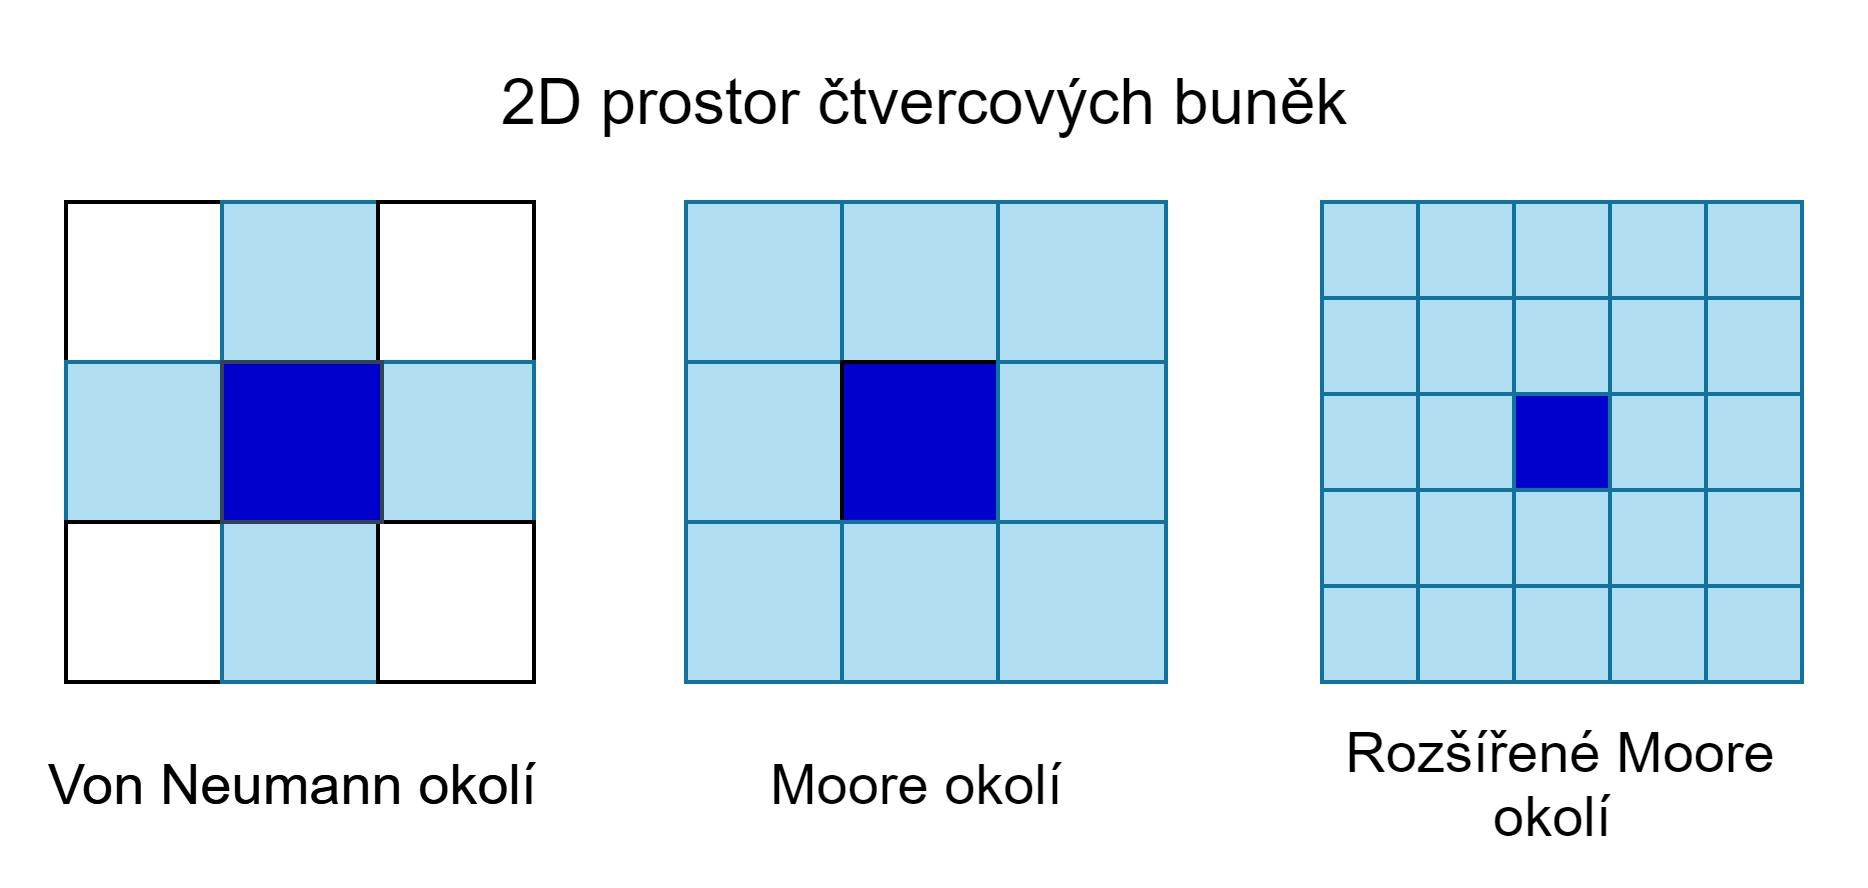
\includegraphics[width=0.65\textwidth]{obrazky-figures/ch2/2D-okoli.png}\hspace{0.5cm}
    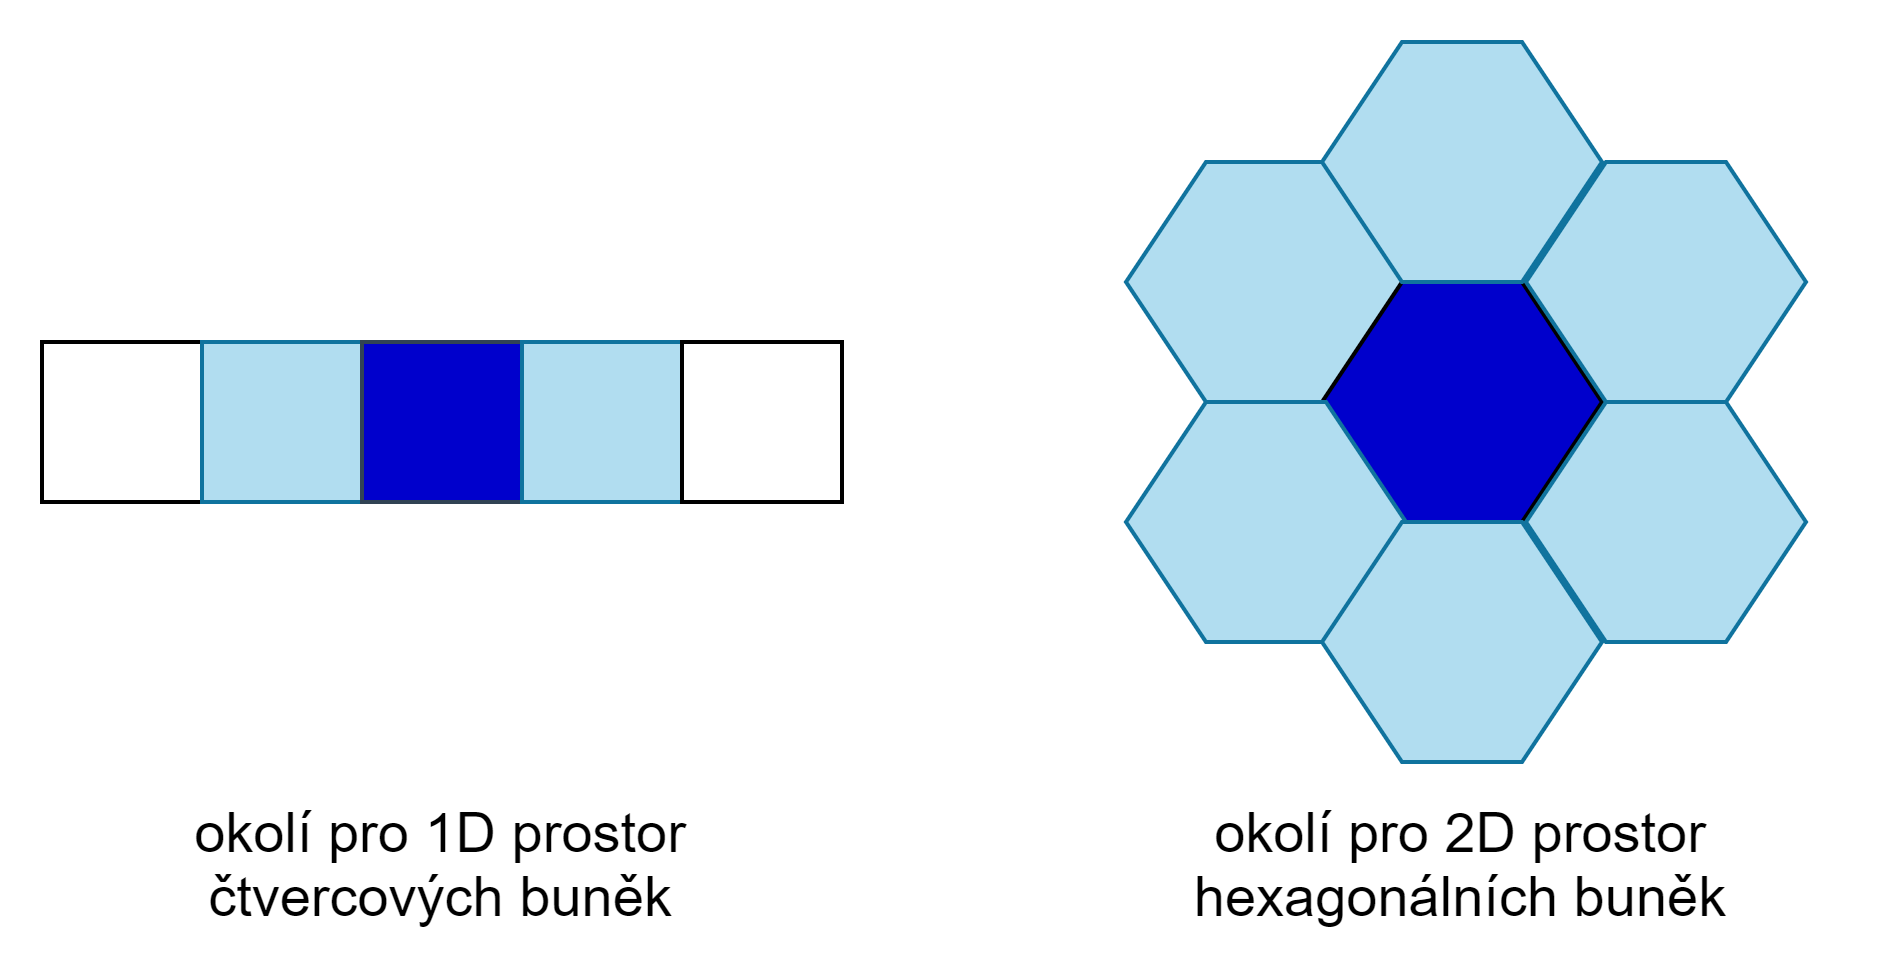
\includegraphics[width=0.65\textwidth]{obrazky-figures/ch2/jina-okoli.png}
    \caption{Příklady okolí (tmavě modrá = zkoumaná buňka, světle modrá = okolí).}
    \label{fig:2D-okoli}
\end{figure}

Jak je již popsáno u formálního popisu, pravidla určují následující stav buňky v čase, který je závislý pouze na jejím aktuálním stavu a stavu jejího okolí, a to pro všechny možnosti vstupu. Pomocí funkce stavu buňky ${s(t)}$ a jejího okolí ${N_s(t)}$ lze vyjádřit rovnici~\ref{eq:CA-rule} pravidla~\cite{ims}.
\begin{equation}
s(t + 1) = f(s(t), N_s(t))
\label{eq:CA-rule}
\end{equation}
Některá pravidla mohou mít i vlastnosti udávající typ pravidlu, které definuje~\cite{mechanics-CA}:
\begin{itemize}
    \item \textbf{totalistic} = o výsledku rozhoduje součet hodnot vstupních buněk (např. Game of Life),
    \item \textbf{legal} = z nulového vstupu nemůže samostatně vzniknout nenulový.
\end{itemize}

\subsection*{Klasifikace}
Stephen Wolfram ve své knize \textit{A New Kind of Science}~\cite{wolfram-NewKindOfScience} definoval 4 třídy pro dělní CA, vypsané níže.
\begin{enumerate}
    \item Téměř všechny počáteční vzory CA se po konečném počtu kroků dostanou do 1 stabilního, homogenního stavu. Zmizí jakákoliv náhodnost v počátečním vzoru.
    \item Téměř všechny počáteční vzory CA se vyvinou do periodicky se opakujících (oscilujících) struktur/stavů nebo zůstane stabilně v některém ze stavů.
    \item Deterministický chaos\,--\,téměř všechny počáteční vzory se vyvíjejí pseudonáhodným, nebo chaotických způsobem. Stabilní struktury, které se objeví jsou rychle zničeny okolním hlukem.
    \item Téměř všechny počáteční vzory se vyvíjejí do struktur, které interagují složitým a zajímavým způsobem, s tvorbou místních struktur, které jsou schopny přežít po dlouhou dobu. Konečným výsledkem mohou být stabilní nebo oscilující struktury typu 2 (k~dosažení může být ale potřeba velký počet kroků). Pod tuto třídu patří Game of Life (viz níže).
\end{enumerate}

Některé celulární automaty lze označovat také jako \textbf{reverzibilní}. Ty jsou definované jako systémy, které neztrácí informaci při svém vývoji v čase\,--\,což znamená, že v každém okamžiku lze otočit vývoj času a navrátit se k předchozím stavům~\cite{ims}. Kvůli jejích chaotickému chování nejsou CA 4. třídy nikdy reverzibilní.

\subsection*{Historie a Game of Life}
Za vznikem celulárních automatů stáli ve 40. letech 20. století matematici John von Neumann a~Stanisław Ulam. Ulam studoval růst krystalů pomocí jednoduché mřížky~\cite{pickover2009math} a~von Neumann řešil modely samoreprodukujících se organismů~\cite{history_CA}. Ulam von Neumannovi navrhl využití diskrétního systému~\cite{schiff2011cellular} s buňkami, které se mění po jednotlivých krocích/iteracích. Na základě dalšího výzkumu došli k vyvinutí základů CA a John von Neumann následně na základě myšlenek celulárních automatů sepsal knihu \textit{Theory of Self-Reproducing Automata}, kde detailně, spolu s důkazy o jeho možné existenci, popisuje jeden z prvních konceptů realistických samo-replikujícího systému, \textit{von Neumannův univerzální konstruktor}~\cite{theory_neumann} který funguje jako univerzální kopírka, která by v teorii replikovala sebe sama pomocí surovin z prostředí, ve kterém se nachází. 
\todo{je to zajímavé ale mám to tu vůbec zmiňovat když to nesouvisí s počítačovýma CA?}

Dalším z důležitých matematiků pro vývoj CA byl John Conway, který v roce 1970 vytvořil pravidla pro \textbf{Game of Life}~\cite{history_CA}, celulární automat na 2D mřížce s buňkami nabývajících 2 stavů\,--\,živá, mrtvá, využívající Moorovo okolí o 8 sousedech (viz obrázek~\ref{fig:2D-okoli}). Pravidly jsou~\cite{Game_Of_Life}:
\begin{itemize}
    \item pokud živá buňka sousedí s 2 nebo 3 živými sousedy přežívá do další generace,
    \item neživá buňka, která má přesně 3 živé sousedy oživne,
    \item zbytek buněk do další generace nepřežívá a stává se mrtvými.
\end{itemize}
I přes svoji jednoduchost tento systém nabývá klasifikace 4. třídy, tedy projevuje náhodnost, ale zároveň se v jeho generacích objevují struktury, které vykazují rozmanité vlastnosti a~dodávající systému částečný řád. Jedním z těchto struktur, je takzvaný kluzák (anglicky \textit{glider}), který se postupem iterací pohybuje po mřížce~\cite{Game_Of_Life}. Ilustraci jeho pohybu je možné vidět na obrázku~\ref{fig:game_of_life}.
\begin{figure}[H]
    \centering
    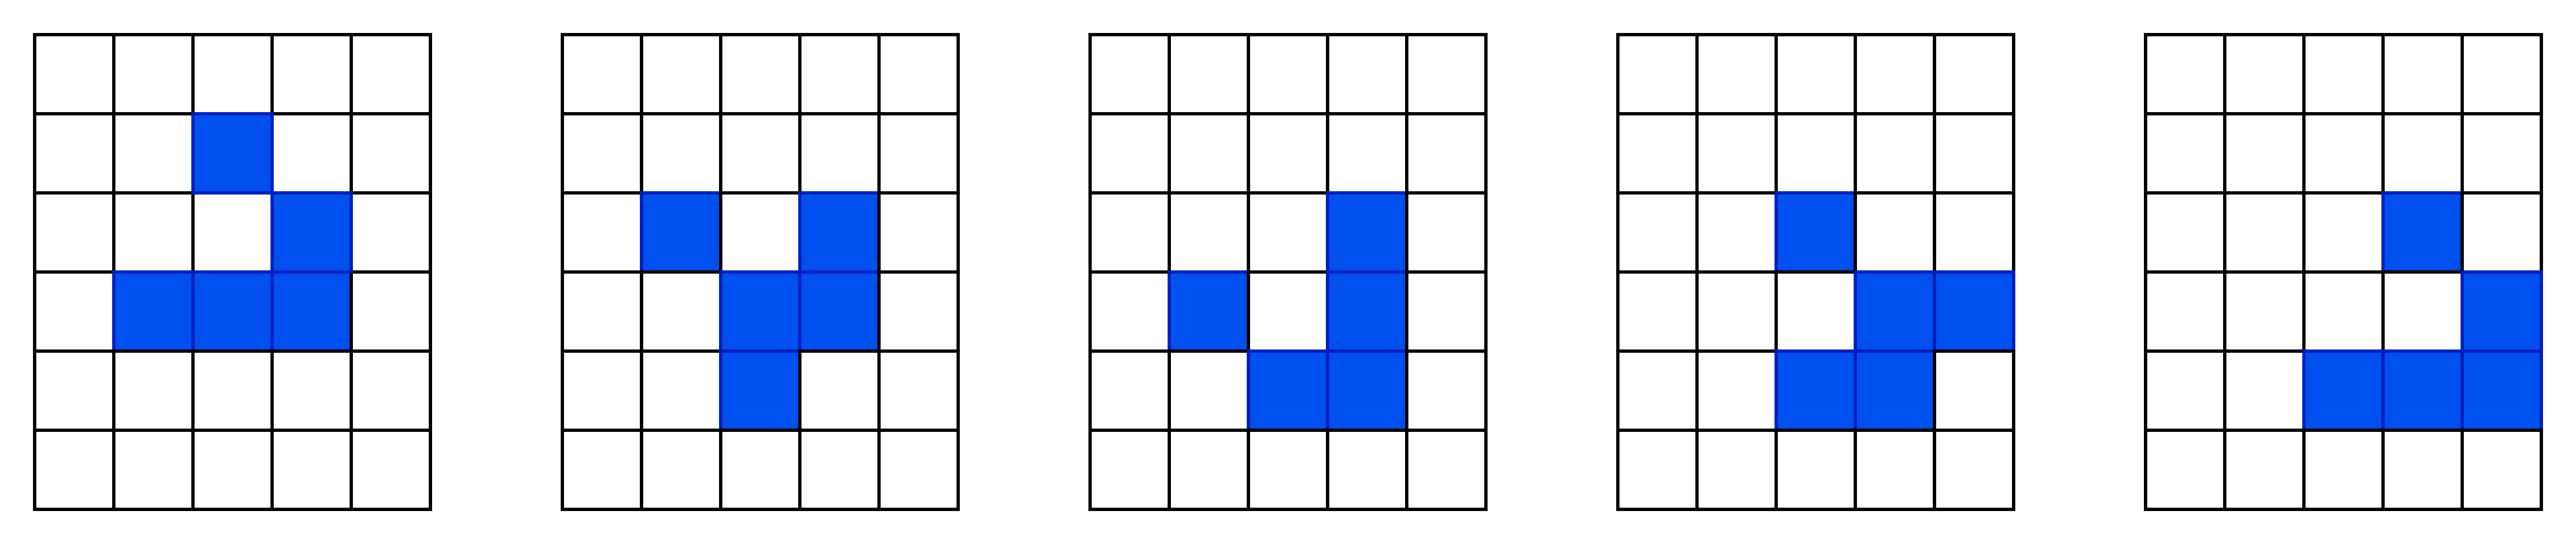
\includegraphics[width=\textwidth]{obrazky-figures/ch2/GameOfLife.png}
    \caption{Pohyb kluzáku/glideru v CA Game of Life.}
    \label{fig:game_of_life}
\end{figure}

\begin{figure}[H]
    \centering
    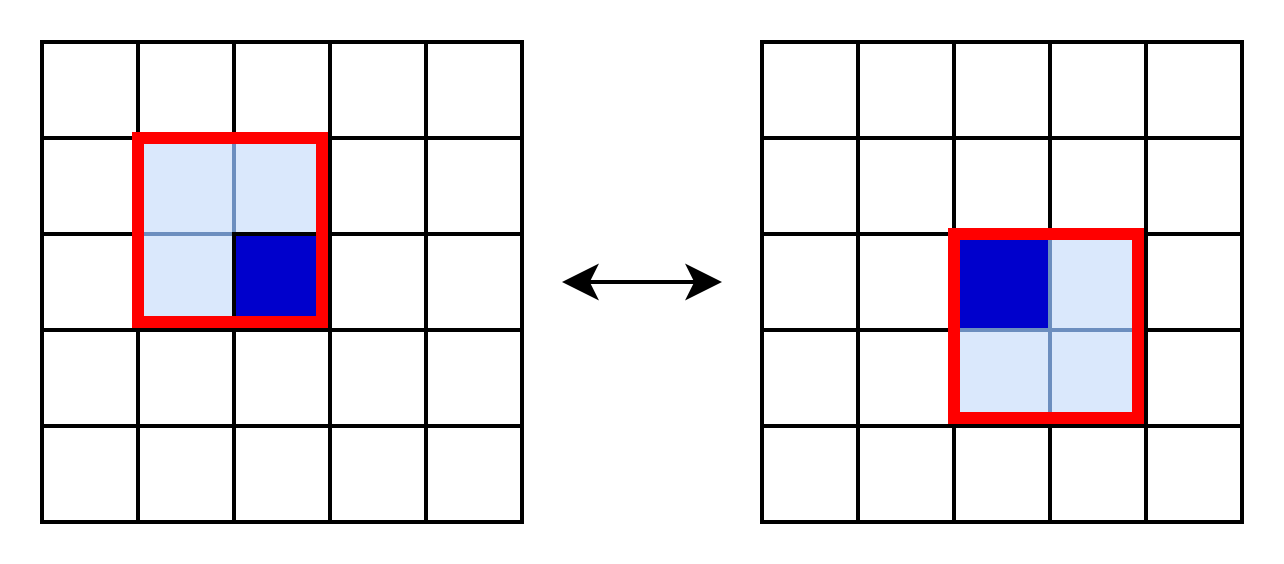
\includegraphics[width=0.6\textwidth]{obrazky-figures/ch2/Margolus.png}
    \caption{Margolusovo okolí (tmavě modrá = zkoumaná buňka, červená = 2x2 blok, světle modrá = okolí).}
    \label{fig:Margolus}
\end{figure}

Posledním, zde zmíněným, důležitým vědcem v historii CA byl Stephen Wolfram, který, jak již bylo zmíněno, ve své knize \textit{A New Kind of Science}~\cite{wolfram-NewKindOfScience} popsal 4 třídy pro klasifikování celulárních automatů a to podle jejich vztahům k druhému na základě fyzikálního zákonu zachování hmotnosti.

\subsection*{Využití celulárních automatů ve hrách}
Jedním z využití CA obsahují hry \uv{padajícího písku}, neboli \textit{Falling-sand games/simulators}. Tyto hry jsou nejčastěji 2D, sandboxové (= podporující kreativitu), jsou založeny například na blokovému/rozdělujícímu celulárnímu automatu, které mohou simulovat reálnou fyziku, jelikož jsou reverzibilní a dodržují fyzikální zákon zachování hmot~\cite{schiff2011cellular}. Nejjednodušší okolí využívané na vyhodnocení těchto CA je Margolusovo (viz obrázek~\ref{fig:Margolus})\,--\,2D mřížka je rozdělena na 2x2 čtverce, které se každou generaci posouvají diagonálně o jednu buňku~\cite{schiff2011cellular} (okolí v čase t se tedy skládá ze všech buněk, které se nacházejí v bloku v aktuálním čase).

\noindent Hráč má při hraní hry přístup k několika materiálům/elementům, které mají každý své vlastní vlastnosti (gravitace, reaktivnost s jinými materiály), se kterými může interagovat na dané ploše. Příkladem těchto her může být The Powder Toy~\footnote{https://powdertoy.co.uk}, The Sandbox (2012), Sandspiel (ukázka na obrázku~\ref{fig:Sandspiel}) či Noita (hra doplněná o roguelike aspekt).
\begin{figure}[H]
    \centering
    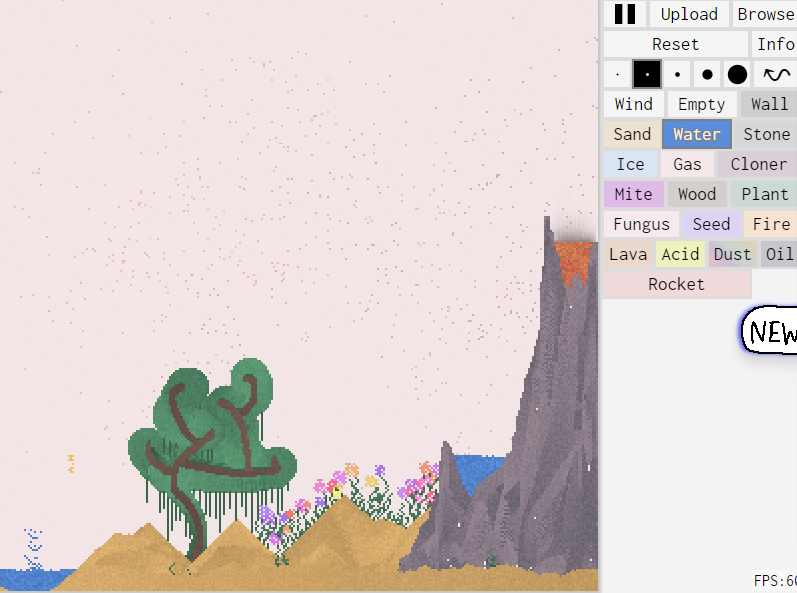
\includegraphics[width=0.5\textwidth]{obrazky-figures/ch2/SandSpiel.png}
    \caption{Ukázka ze hry Sandspiel.}
    \label{fig:Sandspiel}
\end{figure}

\begin{figure}[H]
    \centering
    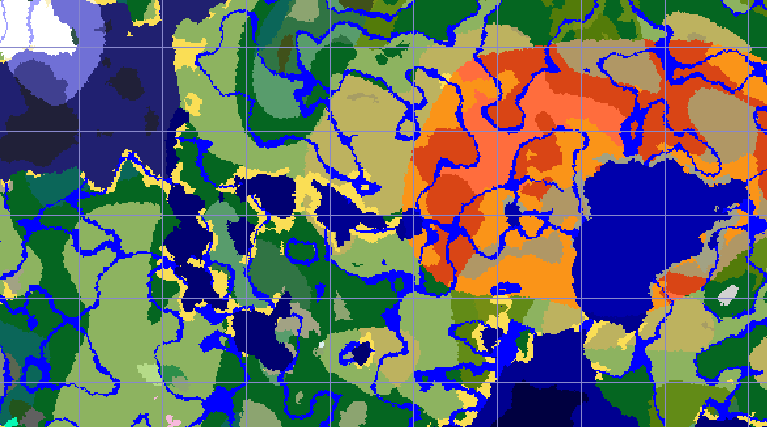
\includegraphics[width=0.7\textwidth]{obrazky-figures/ch2/minecraft_biom.png}
    \caption{Příklad vygenerovaného Minecaft světa s různými biomy}
    \label{fig:minecraft_biom}
\end{figure}

Rozšířenější, a v moderních hrách i častější, je využití CA na procedurální generování terénu\,--\,to je možné najít ve hrách jako je Tje využit u her vyžadujících větší a pestrý svět, či vysoký počet úrovní vyžadujících rozmanité překážky. Je to, jelikož klasické \uv{lidské} výtvory mohou být drahé 2 způsoby. Manuální navrhovaní obrovské mapy, či 100+ úrovní lidmi zabere mnoho času, energie a může naskytnout repetitivita, také tyto před-vytvořené mapy zabírají mnoho paměti a jejich načítaní může být obtížné na procesor\,--\,procedurální generace tedy vytváří mapy za chodu aplikace, takže vyřeší oba problémy~\cite{Procedural_Game_Map}.

Minecraft například generuje základ své mapy díky stochastickým celulárním automatům spuštěných nad zpracovanými (např. pomocí šumu) výsledky kongruentních generátorů~\cite{Minecraft}. Stochaistické/Náhodné celulární automaty, jsou CA u nichž nejsou pravidla deterministická (tj. nepředvídatelná), ale pravděpodobnostní\,--\,to znamená, že místo pevného pravidla určujícího následující stav buňky má zadané pravděpodobnosti možných nových stavů buňky~\cite{DBLP:journals/corr/abs-1304-7185}. Díky tomuto dochází k definování přechodů a prolínání mezi různými poddruhy biomů (příklad vygenerované mapy je vidět na obrázku~\ref{fig:minecraft_biom}). Například teplé oblasti mají 50\% šanci, že se promění v poušť, 33\% v savanu a 17\% v roviny, nebo oceány mající 50\% šanci, že se promění v zem~\cite{Minecraft}.

Některé z jednodušších možností generování prostředí s celulárními automaty je využití algoritmů na náhodné generování jeskyní. Příkladem může být například algoritmus (zapsán níže algoritmem \ref{algo:cave_gen}) z naučné stránky envatotuts+~\cite{CaveCA}, kde buňka CA může nabývat 2 stavů\,--\,živá, mrtvá, jehož výsledek je na obrázku~\ref{fig:cave}.
\begin{algorithm}
\caption{Generování jeskyní pomocí CA}\label{algo:cave_gen}
\begin{algorithmic}[1]
\State \textbf{Input:} $\text{matrix}, \text{row}, \text{col}, \text{deathLimit}, \text{birthLimit}$
\State \textbf{Output:} updated state of the cell
\State $\text{neighbors} \gets \text{countAliveNeighbours}(\text{matrix}, \text{row}, \text{col})$
\State $\text{cellValue} \gets \text{matrix[row][col]}$
\If{$\text{cellValue} = \text{alive}$}
    \If{$\text{neighbors} < \text{deathLimit}$} \Comment{Too many neighbours} 
        \State \textbf{return} $\text{dead}$
    \Else
        \State \textbf{return} $\text{alive}$
    \EndIf
\Else
    \If{$\text{neighbors} > \text{birthLimit}$} \Comment{Reborn} 
        \State \textbf{return} $\text{alive}$
    \Else
        \State \textbf{return} $\text{dead}$
    \EndIf
\EndIf
\end{algorithmic}
\end{algorithm}
\newline
Algoritmus funguje na několika jednoduchých principech, s nimiž je možné různě manipulovat, a to změnou hodnot \verb|deathLimit| a \verb|birthLimit|:
\begin{itemize}
    \item narození = pokud je buňka mrtvá a má určitý počet živých sousedů, v následující iteraci oživí (podpora růstu jeskynních chodeb),
    \item smrt = pokud je buňka živá a má příliš málo mrtvých sousedů, zemře v následující iteraci (vytváření otevřených prostorů v jeskyni),
    \item přežití = pokud je buňka živá a má dostatečný počet živých sousedů, přežívá do následující iterace (udržování existující struktury jeskyní).
\end{itemize}

\begin{figure}[H]
    \centering
    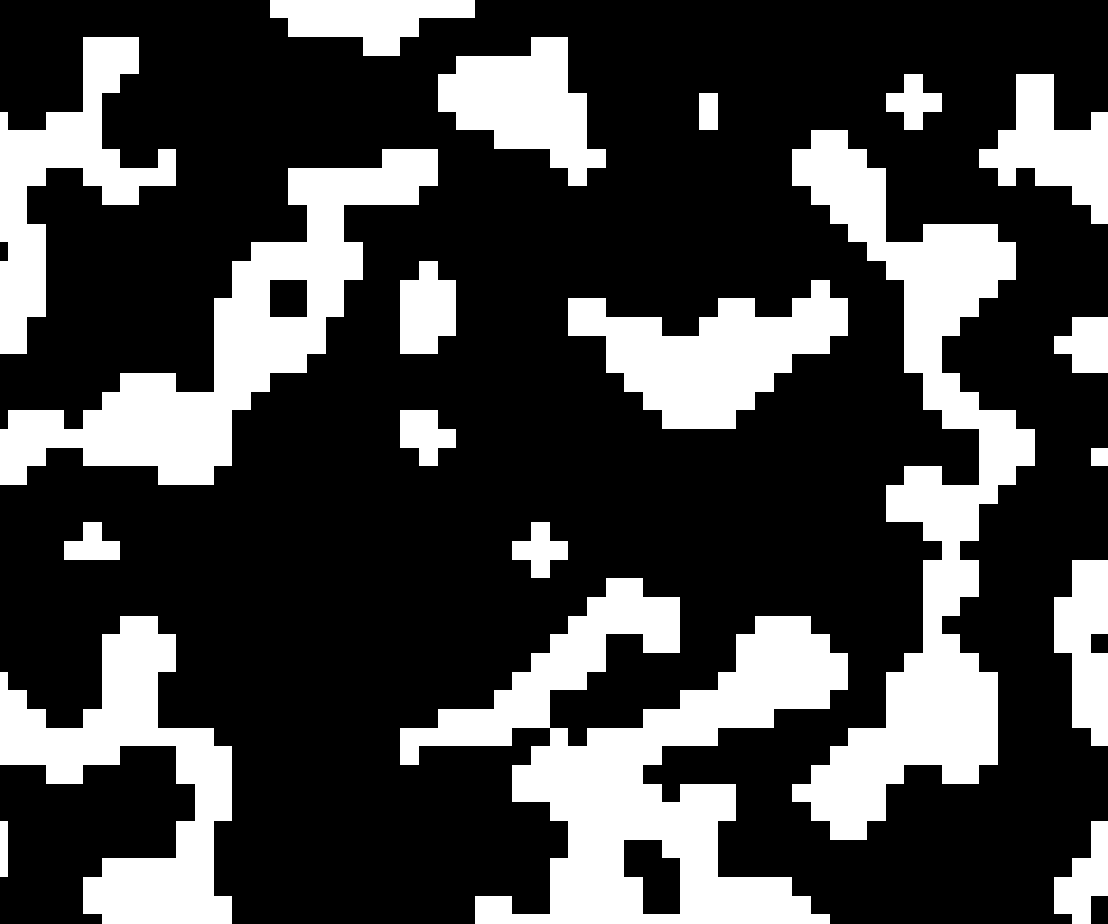
\includegraphics[width=0.5\textwidth]{obrazky-figures/ch2/cave.png}
    \caption{Příklad algoritmu generování jeskyní s využitím Moorova okolí,	deathLimit = 3, birthLimit = 4.}
    \label{fig:cave}
\end{figure}

Také je možné využít algoritmy, generující strukturu podobnou bludišti. Celulárním automatem s touto vlastností je OCA:Maze~\cite{OCA:Maze}. Hlavním principem tohoto algoritmu s~Mooreovým okolím je, že pokud má buňka živých 1 až 5 sousedů tak přežije a ožívá pokud má přesně 3 sousedy\,--\,to znamená, že je pro buňky složitější zemřít a tím se vytváří vzory podobné bludišti, jak je vidět v levé částí obrázku~\ref{fig:OCA:Maze}. Při generování s náhodnou matici, ale nejsou cesty zcela propojené, získáváme jen mnoho nepropojených místností. Existuje i~jeho upravená verze (Mazectric), která ale omezuje počet sousedů potřebný přežití na 1~až~4, díky čemuž vznikají rovnější a delší \uv{cesty}~\cite{OCA:Maze}, což je možné vidět na pravé částí obrázku~\ref{fig:OCA:Maze}.
\begin{figure}[H]
    \centering
    
\includegraphics[width=0.47\textwidth]{obrazky-figures/ch2/OCA:Maze.png}\hspace{0.5cm}
    
\includegraphics[width=0.47\textwidth]{obrazky-figures/ch2/Mazectric.png}
    \caption{Porovnání výsledků CA OCA:Maze (vlevo) a Mazectric (vpravo).}
    \label{fig:OCA:Maze}
\end{figure}
    
%--------------------------
% Prohledávání stavového prostoru
\section{Prohledávání stavového prostoru}
Stavový prostor (anglicky \textit{State space}), využívaný na řešení úloh, lze v informatice popsat jako orientovaný graf, v němž jeho uzly reprezentují stavy, a hrany reprezentují operátory, či stavové přechody~\cite{State-Space_Search}. Formálně je možné stavový prostor a jeho aktuální řešenou úlohu zapsat jakožto čtveřici (S, O, $s_0$, G), jejíž prvky zde definovat jako~\cite{izu}:
\begin{itemize}
    \item S je množina všech možných stavů,
    \item O je množina všech přechodů mezi stavy/operátorů, kterými lze měnit stavy,
    \item $s_0$ je počáteční stav řešené úlohy, $s_0 \in S$,
    \item G je neprázdná podmnožina S cílových stavů úlohy.
\end{itemize}
Úlohy lze řešit díky neinformovaným/slepým metodám, nebo informovaným metodám, které jsou popsány níže. 

\subsection*{Neinformované metody}
Nazývají se neinformovanými neboli slepými, jelikož nemají žádné začáteční informace o~prostoru a umístění cíle. Což znamená, že tyto vyhledávající metody systematicky prohledávají stavový prostor, dokud nenajdou zadaný hledaný výsledek, který do té doby ani neberou v úvahu, pouze pokračují v \uv{prolézání} prostorem~\cite{poole2023artificial} (či neúspěšně prohledají všechny části stavového prostoru). Dále v kapitole jsou popsány některé příklady metod tohoto typu.

\subsubsection*{\textbullet Metoda slepého prohledávání do šířky (BFS)}
Metoda funguje na principu fronty FIFO (\textit{= first-in, first-out}) do které postupně zapisuje uzly, které jsou objeveny, ale neprohledány~\cite{poole2023artificial}. 

\begin{figure}[H]
    \centering
    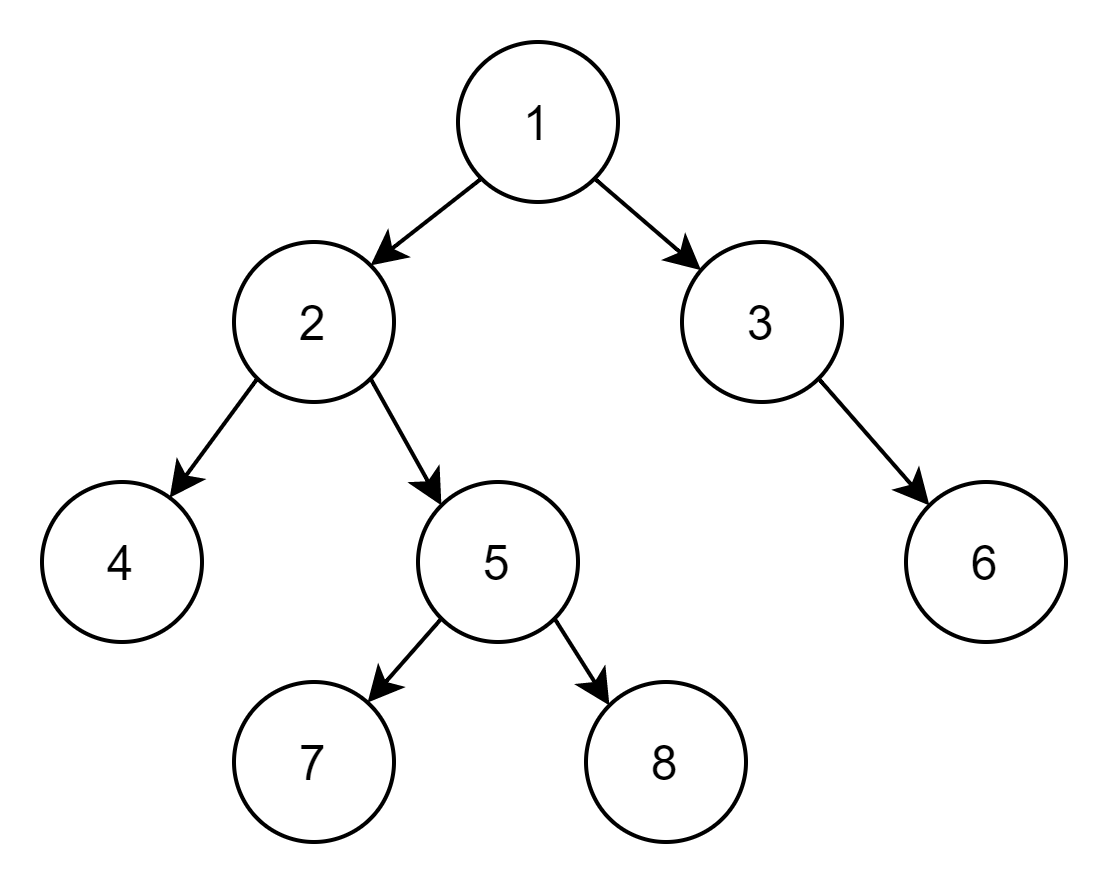
\includegraphics[width=0.48\textwidth]{obrazky-figures/ch2/BFS.png}\hspace{0.25cm}
    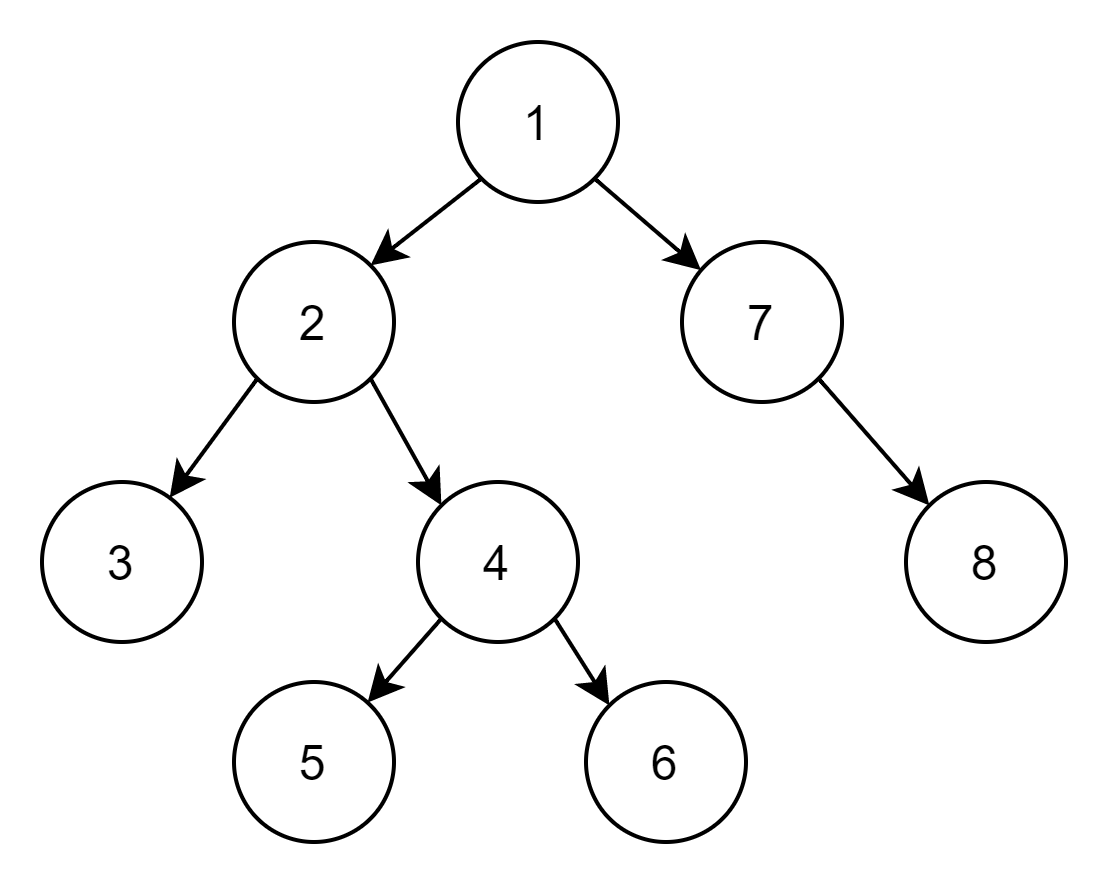
\includegraphics[width=0.48\textwidth]{obrazky-figures/ch2/DFS.png}
    \caption{Porovnání metod prohledávání stavového prostoru BFS (vlevo) a DFS (vpravo).}
    \label{fig:BFS_DFS}
\end{figure}

Prohledávání začíná v kořeni, neboli startovním uzlu, a postupně po úrovních, prochází prvně sousedy kořene, následně sousedy jeho sousedů, atd. dokud nedojde k cíli (zadaný hledaný uzel), od kterého navrátí nejkratší cestu až ke kořeni~\cite{Introduction_to_Algorithms}, či dokud neprohledá neúspěšně celý prostor. Výsledek prohledávání je možné vidět vlevo na obrázku~\ref{fig:BFS_DFS}

Časová složitost je \(\mathcal{O}_{BFS} = |V| + |E|\), kde \(|V|\) je součet počtu uzlů a \(|E|\) je počet hran~\cite{CS225BFSDFS}.

\subsubsection*{\textbullet Metoda slepého prohledávání do hloubky (DFS)}
Metoda pracující se zásobníkem LIFO (\textit{= last-in, first-out}), který využívá k \textit{backtrackingu}, neboli navrácení~\cite{poole2023artificial}. Stejně jako BFS začíná v kořeni, od kterého ale jde do hloubky. To znamená, že vybere jeden neprozkoumaný synovský sousední uzel, u kterého vybere jeho neprozkoumaný synovský sousední uzel a takto pokračuje, dokud nedorazí na \uv{dno}, tedy do místa, kde už nemůže pokračovat hlouběji do dalších sousedů\,--\,v tomto případě se pomoci, již zmíněného, \textit{backtrackingu} navrátí k nejbližšímu otcovskému sousedovi, u kterého ještě nebyly prozkoumány všechny sousedské uzly a prohledává dál~\cite{Introduction_to_Algorithms}. Toto pokračuje, dokud nenajde hledaný cílový uzel, nebo dokud neprojde celý prostor bez nalezení cíle. Ukázka průchodu stromem je v pravé části obrázku~\ref{fig:BFS_DFS}.

Stejně jako u BFS, časová složitost je \(\mathcal{O}_{DFS} = |V| + |E|\), kde \(|V|\) je součet počtu uzlů a \(|E|\) je počet hran~\cite{CS225BFSDFS}.

\subsubsection*{\textbullet Metoda postupného zanořování do hloubky (IDS)}
Tato metoda je kombinací BFS a DFS, což znamená, že prohledávání funguje stejně jako u~DFS s výjimkou, že algoritmus postupuje po úrovních a postupně zvyšuje limit hloubky~\cite{poole2023artificial}. Tedy při první iteraci prohledává hloubkově pouze první úroveň, poté co je celá prohledaná postupuje na druhou iteraci, při které už vstupuje i do druhé atd. dokud nenajde cíl, či nevyčerpá celý stavový prostor. 

IDS se využívá pokud nemůžeme stanovit hloubku řešení a jeho časová složitost je \(\mathcal{O}_{IDS}(b^{d})\), kde \(b\) je faktor větvení (průměrný počet následovníků uzlu) a \(d\) hloubku optimálního řešení~\cite{izu}.

\begin{figure}[H]
    \centering
    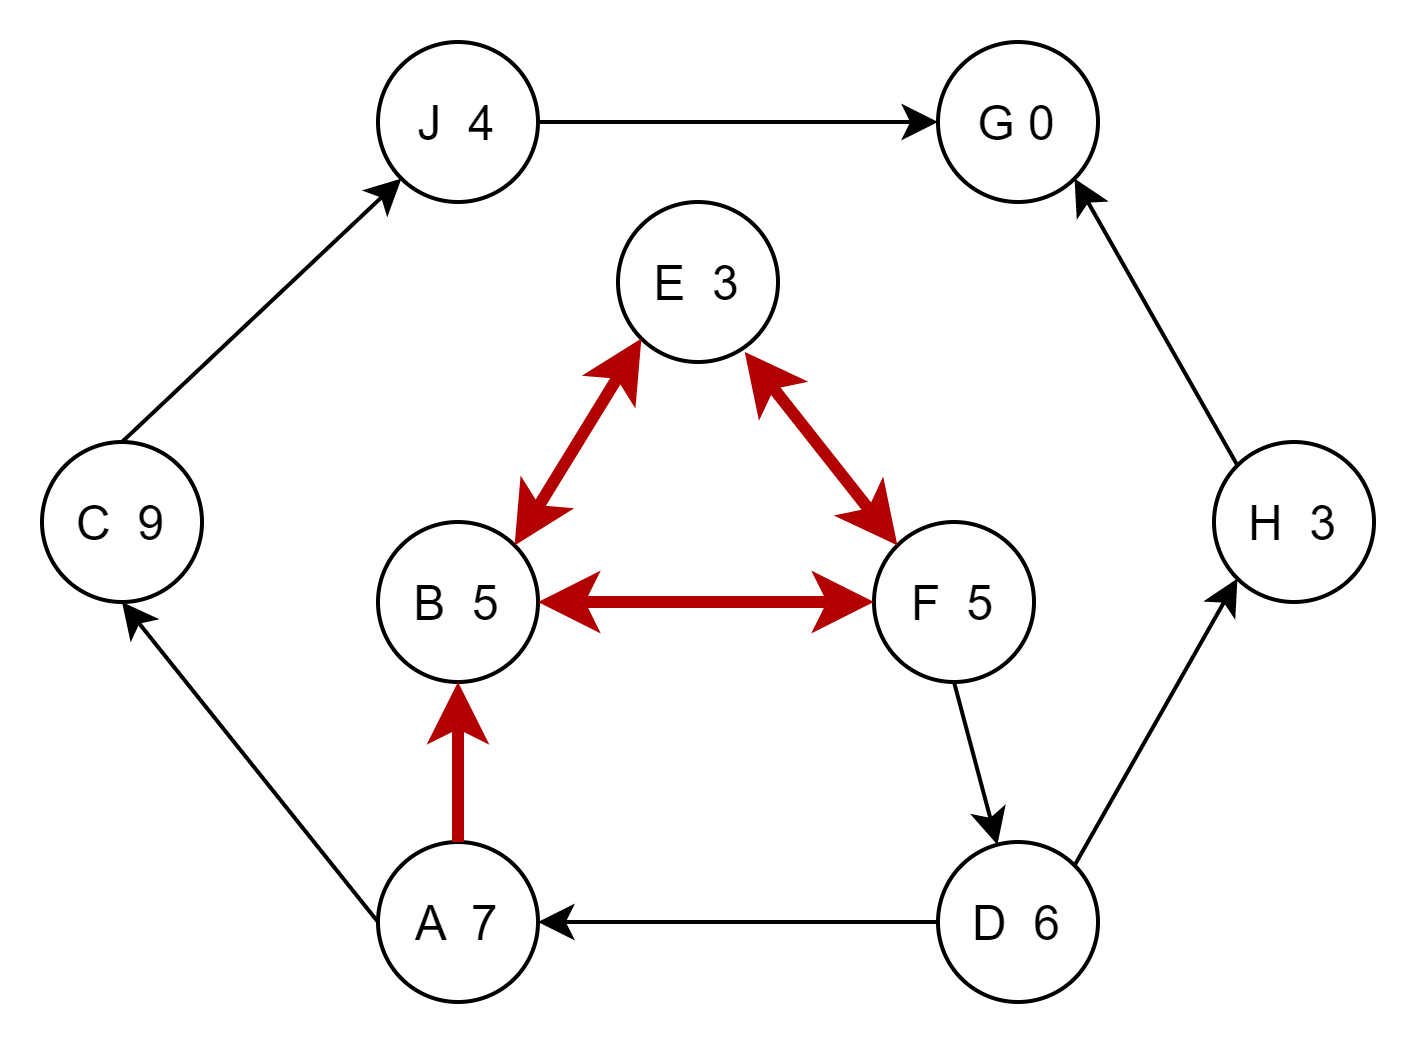
\includegraphics[width=0.7\textwidth]{obrazky-figures/ch2/GreedySearch.png}
    \caption{Nespolehlivost metody hladového prohledávání při hledání cesty z A do G, červeně zvýrazněno cyklení (uzly ve formátu [název uzlu, heuristika]).~\cite{poole2023artificial}}
    \label{fig:GreedySearch}
\end{figure}

\subsection*{Informované metody}
Informované metody na rozdíl od neinformovaných znají polohu cíle~\cite{izu}, kterou využívají na zhodnocení cesty pomocí funkce  ${f(n)}$, kde ${n}$ je stav/uzel. Tyto metody jsou také nazývány heuristickými, jelikož využívají k dosáhnutí cíle heuristickou funkci\,--\,díky této funkci ${h(n)}$ lze vypočítat pomocí uzlu ${n}$ nezáporné reálné číslo značící odhad nákladů na cestu z uzlu ${n}$~do uzlu cílového~\cite{poole2023artificial}. Čím menší je výsledné číslo, tím pravděpodobněji povede k cílovému uzlu a tedy ${h(n) = 0}$, ${n}$ je cílovým uzlem~\cite{AI-Modern_approach}.

\subsubsection*{\textbullet Metoda hladového prohledávání}
Anglicky nazývaný \textit{Greedy search}, je jeden z nejlehčích přístupů, jelikož využívá na zhodnocení uzlu pouze heuristickou funkci, tedy ${f(n) = h(n)}$~\cite{AI-Modern_approach}. Další krok od aktuálního uzlu se rozhoduje pouze v závislosti na této funkci, tedy hrana s nejmenší heuristikou, čímž může dojít k chybnému výsledku\,--\,metoda hladového prohledávání negarantuje nalezení výsledku~\cite{poole2023artificial}. 

Chybný postup k výsledku můžeme vidět v obrázku~\ref{fig:GreedySearch}, na kterém se nachází příklad z knihy \uv{Artificial Intelligence: Foundations of Computational Agents}~\cite{poole2023artificial}, kde při snaze nalezení cesty z uzlu A do uzlu G zůstane algoritmus zacyklen v uzlech B, E, F.

\subsubsection*{\textbullet Metoda A*}
Metoda A* vyhodnocuje další krok na základě hodnotící funkce ${f(n) = g(n) + h(n)}$, kde ${g(n)}$ udává cenu cesty z předešlého do uzlu ${n}$ a ${h(n)}$ je heuristická funkce~\cite{AI-Modern_approach}. 

Pro správnou funkci A* algoritmu je důležité zvolit přípustnou (anglicky \textit{admissible}) heuristiku, což je heuristika, u které cena cesty z uzlu ${n}$ do cílového uzlu nikdy nepřeceňuje cenu ze startovního uzlu k cílovému~\cite{AI-Modern_approach, izu}. Jednou z přípustných heuristik, je přímá euklidovská vzdálenost mezi 2 uzly~\cite{poole2023artificial}, která vhodná na využití u prostorových problémů s přesnými rozměry (např. 2D mřížkový prostor, bez překážek, se 4 povolenými směry - nahoru, dolu, doleva, doprava). Pokud algoritmus při jeho výpočtu dorazí k výsledku heuristické, který by toto nesplňoval, využívá \textit{backtracking} a pokračuje cestu k dalšímu nejlepšímu uzlu.

Podobně jako u metody hladového prohledávání hledá algoritmus cestu po nejmenších hodnotách, ale díky využití kombinace ${g(n)}$ a ${h(n)}$ je algoritmus řazen jako přípustný (vždy, když existuje, vrací optimální řešení)~\cite{poole2023artificial}.
    
%--------------------------
% Rejection sampling
\section{Rejection sampling}
Rejection sampling, či metoda accept-reject (česky přijetí-odmítnutí), je metoda vzorkování využívaná ke generování náhodných proměnných~\cite{thomopoulos2012essentials}. Je jedním z mnoha algoritmů metody Monte Carlo využívána na vzorkování dat ze sofistikované, neboli obtížně vzorkovatelné, distribuce~\cite{Sachdeva_2021}.

Základní myšlenkou rejection samplingu je, že místo přímého vzorkování komplikované funkce f(X) můžeme generovat vzorky pomocí jednodušší distribuce Q(X), ty následně překontrolovat, zda patří do funkce komplikovanější~\cite{ghojogh2020sampling} a na základě toho je přijmout, či pokud do ní nepatří, odmítnout. Vizuální příklad je možné vidět na obrázku~\ref{fig:RA_graph}, který vyobrazuje vzorky vygenerované na základě funkce Q(X). Vzorky nacházející se v území patřící pod funkci f(X) a označené zelenou barvou, budou akceptovány a body mimo (označené žlutě) jsou odmítnuty.

\begin{figure}[H]
    \centering
    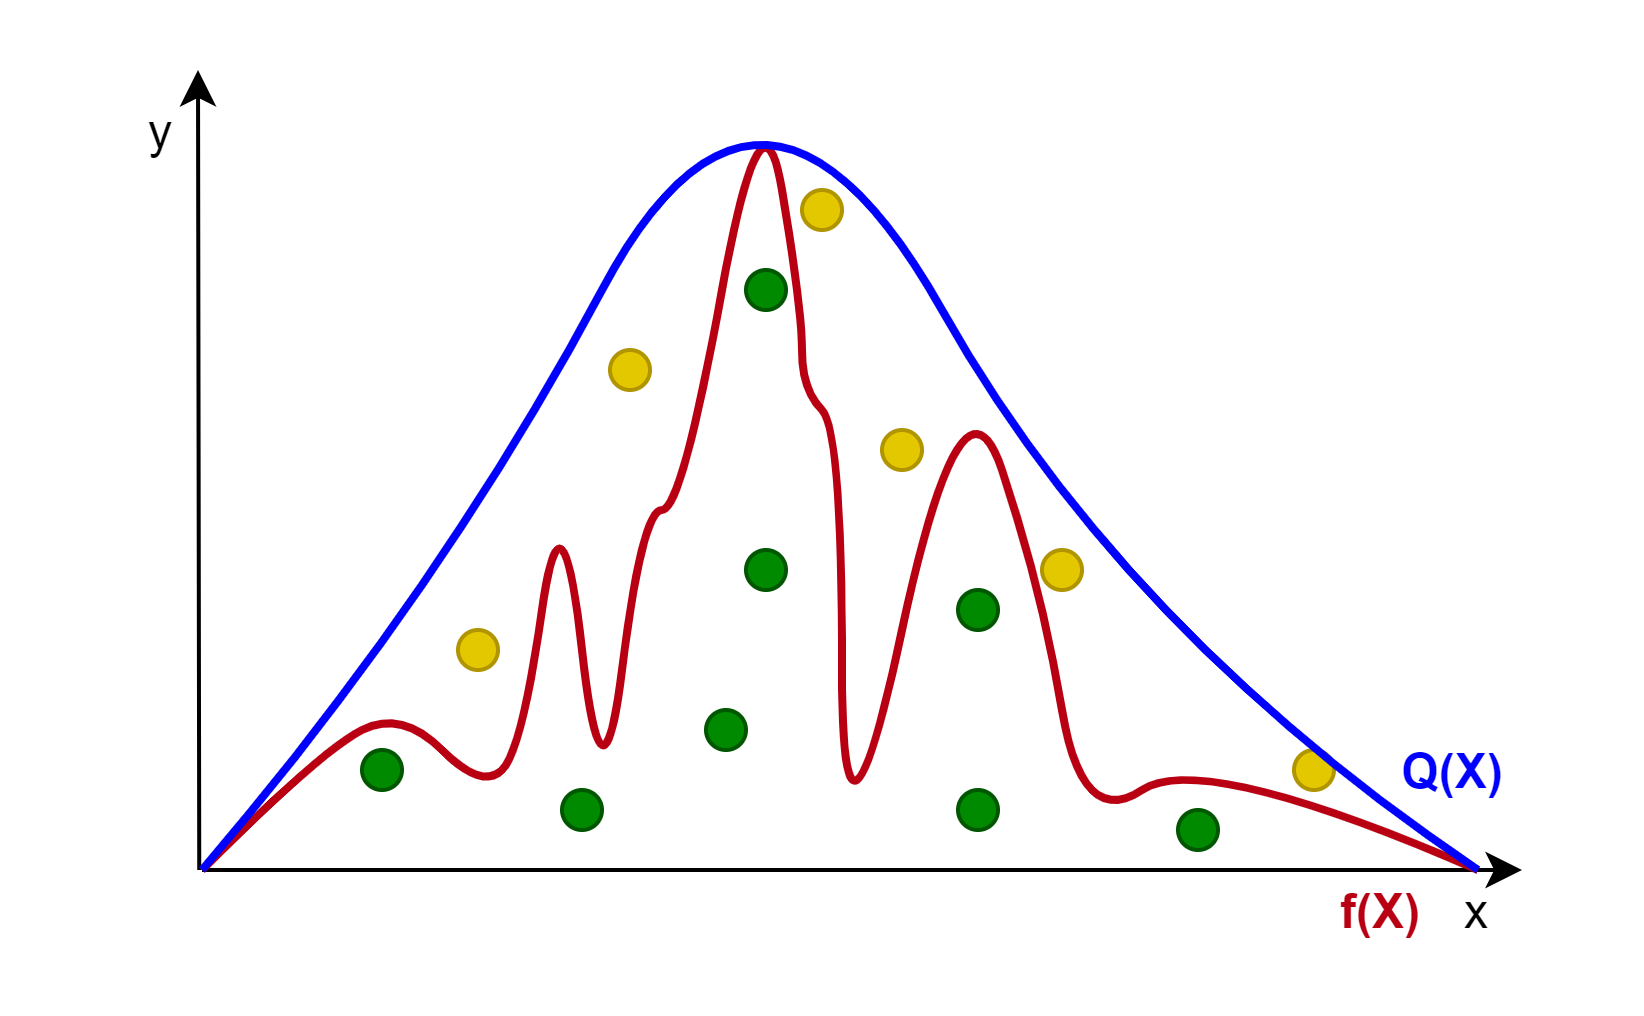
\includegraphics[width=0.9\textwidth]{obrazky-figures/ch2/RA_graph.png}
    \caption{Příklad Rejection samplingu, kde jsou díky využití jednodušší distribuce Q(X) (modrá) získány vzorky ze složitější funkce f(X) (červená)}
    \label{fig:RA_graph}
\end{figure}

Pro detailnější vysvětlení je využit algoritmus~\ref{algo:rejection_sampling} sepsaný podle výukového a literárního přehledu z Univerzity Waterloo~\cite{ghojogh2020sampling} a edukační stránky~\cite{Sachdeva_2021}. V tomto algoritmu je $\mathcal{S}$ sada vzorkovacích dat o velikosti $n$, která se postupně naplňuje generovanými daty, které jsou vzorky složitější funkce f(X). V cyklu generujícím a potvrzujícím vzorky je prvně vytvořen vzorek $x$ z funkce g(X) a následně vzorek $u$ z rovnoměrného rozložení $U(0, c\, g(x_i))$. Škálovací konstanta $c$ je využívána k určení horních mezí pro přijetí nebo odmítnutí vzorku a platí, že $c \cdot g(x) \geq f(x) \ \text{pro všechny } x$.
\label{eq:RA_c}
\begin{algorithm}[h]
\caption{Rejection sampling/Accept-reject}\label{algo:rejection_sampling}
\begin{algorithmic}[1]
    \State \textbf{Input:} $f(x), g(x), c$\;
    \State \textbf{Output:} $\mathcal{S}$
    \State $\mathcal{S} \gets \varnothing$
    \For{$i = 1$ to $n$}
        \State $x_i \sim g(x)$
        \State $u_i \sim U(0, c\, Q(x_i))$
        \If{$u_i < f(x_i)$}
            \State Accept $x_i$: $\mathcal{S} \gets \mathcal{S} \cup \{x_i\}$
        \Else
            \State Reject $x_i$: $i \gets i - 1$
        \EndIf
    \EndFor
\end{algorithmic}
\end{algorithm}

\todo{zeptat se zda vůbec můj kod je rejection sampling}
%===---------------====
% KONCEPT
%===---------------====
\chapter{Koncept 2D labyrintové hry}
\todo{Dopsat - popsat koncept typu her obecně (pravidla labyrintových her,..)}
    
%--------------------------
% Úvod
\section{Úvod do hry/cíle/myšlenka}
\todo{popsat návrh přístupu k problému (zadání), asi taky grafík -> jak jsem postupovala}
%--------------------------
% Mechaniky hry
\section{Mechaniky hry}
\todo{mapa, obecne o hre- princip hry (nekonecna, zvysujici se narocnost)}
\subsection*{Úrovně}
\todo{zvysovani urovni (zde nejaky graf)}
\subsection*{Hráč}
\todo{kamera -> proc jsem vybrala jen cast, ovladani, grafika}
\subsection*{Nepřátelé}
\subsection*{Další objekty}
 
%--------------------------
% Uživatelské rozhraní
\section{Uživatelské rozhraní}
\todo{FIGMA (asi strana plná obrázků + popis proc}

%===---------------====
% IMPLEMENTACE
%===---------------====
\chapter{Implementace 2D labyrintové hry} % TODO NECO KONKRETNEJSIHO
Pro implementaci hry jsem otestovala několik game enginů a zvážila jsem jejich výhody a nevýhody. Jelikož mým cílem bylo vytvořit jednoduchou 2D hru jejíž hlavním a nejsložitějším bodem je mapa vybrala jsem si Godot verzi 4. 

Tuto platformu jsem zvolila oproti jiným možnostem díky její široké a jednoduché podpoře vytváření 2D her, oproti například Unreal Engine, která je zaměřená spíše na realistické 3D světy. Jak je již zmíněno v kapitole o Godotu, tento herní engine na rozdíl od Unity či Unreal Engine využívá vlastní skriptovací jazyk GDScript, podobný syntaxí pythonu, který díky svým knihovnám ulehčuje manipulaci s herními prvky (nodes) a urychluje tak vývoj.

Nejdůležitější vlastností Godotu pro vyváření této hry a její základní mapy byla node "TileMap", která slouží pro vytváření 2D dlaždicových map. Její využití je popsáno v následujících podkapitolách.
    
%--------------------------
% Generování mapy
\section{Generování mapy}
\todo{mock up grafík}
\subsection*{Kostra bludiště}
CA
\subsection*{Propojení bludiště}
GRAFOVÉ ALGORITMY

%--------------------------
% Hráčská postava a její umístění
\section{Cesta bludištěm} % start + cil

%--------------------------
% Experimenty s generováním map pomocí CA
\section{Experimenty s generováním map} % statistiky, proc jsem vybrala dany postup
\todo{statistiky v generovani mistnosti, po propojeni obsah zdi vs cest + kolik CA generaci na plno - jak na kolika, proc, rovnice}

%--------------------------
% Nepřátelé, objekty a jejich rozmístění
\section{Nepřátelé, objekty a jejich rozmístění}

%--------------------------
% Úrovňový systém
\section{Úrovňový systém}

\subsection*{Skóre}

%===---------------====
% TESTOVANI
%===---------------====
\chapter{Uživatelské testování}
Uživatelské testování bylo prováděno formou online anonymního dotazníku (Google Forms), který testované subjekty vyplnily po otestování alfa verze hry. Hra byla testována na počítačích s Windows a Linux operačními systémy. Testery byli aktivní i nezkušení hráči her, naverbováni primárně díky sdílení testovacích prostředků na sociálních sítích.

%--------------------------
% Dotazník
\section{Dotazník}
Otázky jsem vytvářela tak, abych protestovala hlavní aspekty vytvořené hry, kterými jsou její hratelnost, uživatelské rozhraní, stabilita programu a celková náročnost hry. Byla jsem připravena prvky těchto aspektů následně, na základně zpětné vazby, upravit, či předělat aby vyhovovaly požadavkům testerů. Vzhledem k tomu, že byl dotazník vypracován pro hromadné testování, jsou otázky formulovány tak, aby umožňovaly spíše výběr z předem definovaných možností, než aby vyžadovaly volné textové odpovědi, a to kvůli jednoduššímu vyhodnocování. \\
\newline
\noindent Seznam otázek:
\begin{enumerate}
\item Kolik času jste strávili u hraní?
\item Jaká byla vaše nejvyšší dosažená úroveň (level)?
\item Jaký je váš celkový dojem ze hry?
\item Jak byste ohodnotili uživatelské rozhraní a celkovou přehlednost hry?
\item Jak byste ohodnotili stabilitu a výkon hry (záseky/pády, \ldots)?
\item Co pro vás bylo nejtěžší?
\item Jak byste ohodnotil vyváženost zvyšující se obtížnosti?
\item Pokud jste hodnotili hru jako spíše nevyváženou, jaký k tomu byl důvod? (vyberte co platí, popřípadě doplňte)
\item Jaké další funkce/vlastnosti/prvky byste ve hře ocenili/změnili?
\end{enumerate}

%--------------------------
% Analýza výsledků
\section{Analýza výsledků}
Byly získány odpovědi od ... subjektů, kompletní výpis všech odpovědí je přístupný v příloze~\ref{chap:user_testing}.
\subsection*{Hratelnost}
\subsection*{Uživatelské rozhraní}
\subsection*{Stabilita programu}
\subsection*{Náročnost}

%--------------------------
% Závěr testování
\section{Závěr testování}
\subsection*{Implementované změny}

%===---------------====
% ZAVER
%===---------------====
\chapter{Závěr}
\todo{Dopsat - az na konci}
%===============================================================================

% Pro kompilaci po částech (viz projekt.tex) nutno odkomentovat
%\end{document}
